\documentclass[a4paper,11pt]{article}
\usepackage[brazilian]{babel}
\usepackage[utf8]{inputenc}
\usepackage[T1]{fontenc}
\usepackage{epsfig}
\usepackage{array}
\usepackage{pifont} 

\usepackage{scrextend}

\usepackage{graphicx, url}
\usepackage[usenames]{color}
\usepackage{rotating}
\usepackage{url}
\usepackage{pdfpages}
\usepackage{subfigure}
\usepackage[table]{xcolor}
\usepackage{xspace}
\usepackage[verbose, dvips=true, pdftex=false, vtex=false, paperwidth=210mm,paperheight=295mm,top=35mm,left=30mm,bottom=35mm,right=30mm]{geometry}
\usepackage[authoryear]{natbib}
\usepackage{fancyhdr}
\usepackage{setspace}
\usepackage{lscape}

\usepackage{listings}
\lstdefinelanguage{Xtext}{
 morekeywords={grammar, with, hidden, generate, as, import, returns, current, terminal, enum, ID},
 keywordstyle=[1]{\textbf},
 morecomment=[l]{//}, 
 morecomment=[s]{/*}{*/}, 
 morestring=[b]",
 tabsize=2}
 
\newcommand{\lstXtext}[1]{\lstinline[breaklines=true,language=Xtext,basicstyle=\listingsfontinline,mathescape,literate={\-}{}{0\discretionary{-}{}{}}]\S#1\S}

\DeclareGraphicsExtensions{.png,.jpg,.pdf,.mps}
\bibliographystyle{icmc2}

\clubpenalty=10000
\widowpenalty=10000
\newcommand{\rev}[1]{{\color{red}#1}}

\newcommand{\titlehd}{\sffamily\bfseries\selectfont \scriptsize Uma Abordagem de Reestruturação de Sistemas Baseada em Requisitos de Qualidade Pré-Estabelecidos }

\pagestyle{fancy}
\headheight 61pt
\fancyhead{}
\fancyhead[LO]{\epsfig{file=icmc.jpg,height=15mm}}
\fancyhead[RO]{}
\fancyfoot{}

\begin{document}

\begin{center}
\vspace*{1cm}
{\fontsize{17.28}{20}\sffamily\bfseries\selectfont Uma Abordagem de Reestruturação de Sistemas Baseada em Requisitos de Qualidade Pré-Estabelecidos \\\ \\

\small{RELATÓRIO CIENTÍFICO PARCIAL - 01/05/2013 a 28/02/2015}\\ \
\textsf{Apresentado à Fundação de Amparo à Pesquisa do Estado de São Paulo - FAPESP}
 \\
\vspace{3cm}}


\begin{table}[!th]
  \begin{center}
    \begin{tabular}{ll}

	  Número do Processo:      &   FAPESP 2012/05168-4     \\
      Período:        &  Maio/2013 a Fevereiro/2015                    \\
	                   &                                \\
      Bolsista:           &   Rafael Serapilha Durelli (rdurelli@icmc.usp.br)                                     \\
	  
	  \vspace{0.6cm}
      Orientador:        &  Prof. Dr. Márcio Eduardo Delamaro (delamaro@icmc.usp.br)                                           \\

	         &                              \\
	          &  \\
                       &                                  \\
       &                                       \\
              &                                             \\ \\
      \vspace{1cm}

    \end{tabular}
  \end{center}
\end{table}

\vfill
{\fontsize{18}{20}\sffamily\bfseries\selectfont USP - São Carlos \\ Janeiro de 2012}

\end{center}

\vspace{3cm}

\pagebreak
\fancyhead[RO]{\titlehd}
\fancyfoot{\centerline{\thepage}}
\setcounter{page}{1}

\parskip 6pt

\doublespacing
\begin{abstract}

 Relatório Científico Parcial apresentado à Fundação de Amparo à Pesquisa do Estado de São Paulo (FAPESP) com o objetivo de elucidar as atividades realizadas  
 pelo bolsista Rafael Serapilha Durelli durante o segundo período de vigência da bolsa concebida sob o Processo Número 2012/05168-4. 
 O referido período teve inicio em Maio de 2013 e foi finalizado em Fevereiro de 2015. 
 Além disso, este relatório também descreve as atividades que foram finalizadas, as atividades que estão em andamentos, bem como as atividades a serem realizadas no próximo período. 
%01/05/2013 a 28/02/2015
%
Durante o período de vigência anterior, o bolsista conduziu atividades voltadas principalmente à obtenção de uma ampla visão da literatura científica sobre os principais temas de pesquisa relacionado ao projeto em questão. Para tal, uma revisão sistemática foi conduzida. Os resultados da revisão forneceram evidências que suportam e motivam a realização do projeto proposto. A condução da revisão sistemática bem como os principais resultados foram apresentados no relatório anterior.
%
Vale ressaltar que no segundo período de vigência da bolsa, correspondente a este relatório, cinco principais atividades foram conduzidas. Tais atividades são: (\textit{i}) redação de artigos, (\textit{ii}) adaptação de um catalogo de refatoração para o metamodelo Knowledge Discovery Metamodel (KDM), (\textit{iii}) implementação de uma ferramenta semi-automática que fornecer suporte ao catalogo de refatoração adaptado para o KDM, (\textit{iv}) criação de um metamodelo de refatorações, padronizado que contenha características similares ao KDM, ou seja, independente de plataforma e linguagem, com o principal objetivo de auxiliar o engenheiro de modernização durante a elaboração de refatorações e (\textit{v}) definição de uma Linguagem Especifica de Domínio (do inglês Domain-Specific Language - DSL) para auxiliar a instanciação do metamodelo de refatoração. Esse relatório apresenta as atividades desenvolvidas no período de Maio/2013 a Fevereiro/2015.
%
%Software é um produto que tende a evoluir constantemente com o intuito de satisfazer às necessidades de seus usuários. Para isso é necessário submetê-lo a constantes atividades de manutenção, que podem ocasionar um possível degradação no código-fonte. Dessa forma, o objetivo desta proposta de doutorado é o desenvolvimento de uma abordagem que auxilie o engenheiro de software a escolher o melhor conjunto de transformações para um sistema legado com base em requisitos de qualidade pré-estabelecidos e com isso possa identificar o impacto que tais transformações irão ocasionar no sistema legado. Isto é, a abordagem deverá indicar conjuntos de possíveis transformações para a evolução do sistema legado, além disso, deverá informar ao engenheiro o quanto tais transformações irão afetar a evolução/estrutura desse sistema. Com isso, o engenheiro de software poderia previamente escolher qual o melhor conjunto de  transformação se aplica dado um requisito de qualidade pré-estabelecido. Após a escolha das transformações a abordagem também deverá realizar automaticamente tais transformações a fim de reestruturar o sistema legado em um novo sistema. Será avaliado a abordagem por meio de experimentos controlados.

\end{abstract}


      



\section{Introdução}
	 Este relatório tem por objetivo apresentar as atividades realizadas pelo bolsista Rafael Serapilha Durelli durante o período de Maio/2013 a Fevereiro/2015,
 referente à bolsa de doutorado concebida pela Fundação de Amparo à Pesquisa do Estado de São Paulo (FAPESP) sob o Processo Número 2012/05168-4. 
 
 É importante salientar que o trabalho em questão tem sido desenvolvido no Departamento de Ciências da Computação e Estatística do Instituto de Ciência 
 Matemáticas e de Computação (ICMC) da Universidade de São Paulo (campos São Carlos/SP).  
 Este trabalho se insere no contexto do grupo de pesquisas em Engenheira de Software, sob a orientação do Prof. Dr. Márcio Eduardo Delamaro.
 Além disso, é importante salientar que este trabalho esta sendo executado em colaboração com o grupo de engenharia de software da Universidade Federal de São Carlos (UFSCAR)\footnote{http://dc.ufscar.br}.  
 Mais especificamente em colaboração com o Prof. Dr. Valter Vieira de Camargo\footnote{http://buscatextual.cnpq.br/buscatextual/visualizacv.do?id=S819089},
 o qual tem grande experiência na área de engenharia de software com ênfase no desenvolvimento de frameworks no contexto da programação orientada a aspectos e reuso de software.  Ressalta-se que o bolsista criou um vínculo científico com o \textit{Institut National de Recherche en Informatique et en Automatique} (INRIA),  
onde realizou um ano de doutorado sanduíche sobre orientação do  
 Prof. Dr. Nicolas Anquetil\footnote{http://rmod.lille.inria.fr/web/pier/team/Nicolas-Anquetil} o qual tem grande experiência na área de manutenção e reengenharia de software. O doutorado sanduíche em questão foi realizado em Maio de 2013 até Março de 2014.

Durante o período concernente a este relatório, o bolsista dedicou-se às atividades técnicas requeridas para concretização do seu projeto de doutorado bem com às atividades exigidas pelo Programa de Pós-Graduação em Ciências de Computação e Matemática Computacional do ICMC\footnote{Destaca-se que algumas atividades já foram reportadas no relatório anterior}. Considerando as atividades técnicas previstas no cronograma para o período vigente, todas foram devidamente realizadas ou estão progredindo de acordo com o estipulado, a saber: (\textit{i}) redação da monografia e aprovação no exame de qualificação, (\textit{ii}) implementação da abordagem proposta no exame de qualificação, (\textit{iii}) redação de artigos. O exame de proficiência em língua inglesa, exigido pelo Programa de Pós-Graduação do ICMC, foi devidamente realizado e uma pontuação satisfatória foi obtida.

Neste relatório enfatiza-se adaptação de um catalogo de refatoração para o metamodelo \textit{Knowledge Discovery Metamodel} (KDM). Além disso, neste relatório também é enfatizado a implementação de uma ferramenta semi-automática que fornecer suporte ao catalogo de refatoração adaptado para o KDM. Em seguida é apresentado a criação de um metamodelo de refatorações, padronizado que contenha características similares ao KDM, ou seja, independente de plataforma e linguagem. E a definição de uma Linguagem Especifica de Domínio (do inglês Domain-Specific Language - DSL) para auxiliar a instanciação do metamodelo de refatoração.

\textbf{Organização do relatório}


%\section{Plano de Trabalho}\label{plano_trabalho}
%	Hoje em dia diversas companhias estão enfrentando problemas de gerenciamento, manutenção e/ou troca (de parte) de um sistema existente. Esses sistemas geralmente são caracterizados como sistemas legados (SL). SL geralmente são aplicações de grande porte que possuem um papel crucial e importante no contexto de gerenciamento de informação de companhias. Melhorar a compreensão desses SLs (e.g., arquitetura, características, acoplamento, modularização, etc ) é o fator principal durante a evolução/modernização desses sistemas. O processo de obtenção de uma representações de alto nível de um determinado SL é chamado de Engenharia Reversa (ER).

Diferentemente da Engenharia Avante (EA), a ER é comumente definida como o processo de examinar um SL para representa-lo formalmente em um modelo de alto nível de abstração~\citep{Reverse_engineering_and_Design_Recovery_A_Taxonomy}. O principal objetivo para realizar esse processo é para facilitar o entendimento do estado atual do SL. Por exemplo, utilizando esse modelo de alto nível de abstração é possível corrigir possíveis erros, adicionar novas características, reutilizar partes do SL em outros sistemas, ou até mesmo moderniza-lo completamente~\citep{Griffith2011}. De acordo com~\cite{Achievements_and_Challenges_in_Software_Reverse_Engineering}, isto está acontecendo com mais frequência nos dias atuais, em função da necessidade de não só satisfazer novas exigências e expectativas dos usuários, mas também para a adaptação dos SLs para modelos de negócios emergentes, aderindo à mudança da legislação, lidar com a inovação tecnológica (frameworks, \textit{Application Programming Interface} (API), ambientes de desenvolvimento, etc) e ainda preservar a estrutura do sistema para que o mesmo não se deteriore.

Claramente, uma vez que a ER é um processo demorado e sujeito a erros, qualquer solução que auxilie (semi)automaticamente o processo de ER traria ajuda para os engenheiros de software/modernização e, assim, facilitaria sua utilização~\citep{ADMCHAPTERR, ADMBook}. No entanto, essa solução teria de enfrentar vários problemas, a saber: (\textit{i}) Heterogeneidade técnica dos sistemas legados; (\textit{ii}) Complexidade estrutural destes sistemas legados; (\textit{iii}) Escalabilidade da solução desenvolvida; e (\textit{iv}) Adaptability/portability of this solution.

Na década de 90 algumas pesquisas tinha como intuito desenvolver soluções (semi)automática para auxiliar a ER. No entanto, tais soluções eram focadas em tecnologias orientadas a objectos (OO)~\citep{Software_Reuse_and_Reverse_Engineering_in_Practice}. Também surgiu-se o interesse em processos e ferramentas para auxiliar a compreensão de programas desenvolvidos em OO. Entre muitas propostas, algumas focaram na extração e análise de informações relevantes a partir do código fonte ou componentes de software~\citep{Re2_Reverse_engineering_and_reuse_re_engineering}, enquanto outras focaram em banco de dados relacionais~\citep{An_approach_for_reverse_engineering_of_relational_databases}, código compilado ou arquivos binários~\citep{Reversing_Secrets_of_Reverse_Engineering}, etc. No entanto, estas pesquisas eram bastante específicas para uma tecnologia em particular ou um determinado cenário de ER (por exemplo, migração técnica, análise de software).

Com o surgimento de \textit{Model-Driven Engineering} (MDE)~\citep{Model_Driven_Engineering}, suas diretrizes e técnicas fundamentais tem sido utilizadas para auxiliar a construção de soluções eficazes de ER, ou seja, \textit{Model-Driven Reverse Engineering} (MDRE). MDRE formaliza as representações (modelos) derivadas de SL para garantir um entendimento comum sobre o seu conteúdo. Estes modelos são então utilizados como ponto de partida para a ER. Dessa forma, MDRE beneficia diretamente da extensibilidade, da cobertura, reutilização, integração e automação das tecnologias MDE para fornecer um bom suporte para a ER. No entanto, ainda há uma falta de soluções completas destinadas a cobrir processos MDRE completos.

Neste contexto, em 2003 a \textit{Object Management Group} (OMG) criou uma força tarefa para analisar e evoluir os tradicionais processos de ER, formalizando-os e fazendo com que eles fossem totalmente apoiados pelas diretrizes e princípios de MDE. Logo, o termo Modernização Dirigida à Arquitetura (\textit{Architecture-Driven Modernization} - ADM) surgiu como uma solução para os problemas de padronização. A ADM é um processo de modernização de SL que utiliza um conjunto de metamodelos para representar complemente um sistema por meio de diferentes representações arquiteturais. Esses modelos são então submetidos à refatorações e otimizações e o código-fonte é então gerado novamente. Durante a modernização de um sistema são gerados vários modelos de acordo com os metamodelos da ADM, que representam diferentes partes do sistema, como: fluxos de dados, banco de dados, elementos de programação (métodos, classes, tipos de dados, etc.) e arquitetura~\citep{Information_Systems_Transformation_Architecture_Driven_Modernization_Case_Studies, Software_modernization_by_recovering_Web_services_from_legacy_databases}.

O \textit{Knowledge Discovery Metamodel} (KDM) é o principal metamodelo da ADM com uma ampla quantidade de metaclasses, cobrindo desde os níveis mais baixos de abstração de um sistema, como o código-fonte, até níveis mais altos, permitindo a representação de conceitos de qualquer domínio. A idéia principal da ADM é que a comunidade comece a desenvolver ferramentas que atuem somente sobre instâncias do KDM, ao invés de serem dependentes de plataformas e linguagens específicas. Por exemplo, um catálogo de refatorações para o KDM~\citep{iri_catalogue_of_refactoring_2014}\footnote{No periodo de vigência pertinente a esse relatório, um artigo descrevendo um Catalogo de Refatoração Adaptado para o KDM foi publicado em um evento qualis B2 voltado para Engenharia de Software} tem o poder de reestruturar um sistema independentemente da linguagem de programação que foi usada em seu desenvolvimento, uma vez que as refatorações ocorrem em nível do KDM, ou seja, um modelo independente de plataforma e/ou linguagem. 

Sistemas Legados precisam ser refatorados durante toda a sua vida útil para se adequem a novos requisitos. No entanto, geralmente a má aplicação de refatorações/modernizações em SLs pode causar desvios arquiteturais. Embora refatoração (tanto de baixa granularidade quanto alta granularidade) seja um técnica poderosa, e uma atividade recorrente durante a modernização  em SLs, foi constatado durante a condução de um mapeamento sistemático~\citep{iri_systematic_mapping_ADM_2014}\footnote{No periodo de vigência pertinente a esse relatório, um artigo descrevendo um Mapeamento Sistemático foi publicado em um evento qualis B2 voltado para Engenharia de Software} 
que a versão original da ADM, e consequentemente do KDM, não fornecem apoio (por exemplo, a catálogos de refatoração, a metamodelos para definir refatorações, etc) para tal atividade. Além disso, dificilmente a arquitetura de um sistema legado permanece intacta depois de anos de manutenção, isso é, sua arquitetura atual possivelmente é diferente da arquitetura que foi previamente planejada. ADM também não fornece apoio à checagem de conformidade entre a arquitetura planejada e a atual.

Nesse sentido, este relatório enfatiza-se a quatro principais atividades, a saber: (\textit{i}) adaptação de um catalogo de refatoração para o metamodelo KDM, (\textit{ii}) implementação de uma ferramenta semi-automática que fornecer suporte ao catalogo de refatoração adaptado para o KDM, (\textit{iii}) criação de um metamodelo de refatorações, padronizado que contenha características similares ao KDM, ou seja, independente de plataforma e linguagem, com o principal objetivo de auxiliar o engenheiro de modernização durante a elaboração de refactorações e (\textit{iv}) definição de uma Linguagem Especifica de Domínio (do inglês Domain-Specific Language - DSL) para auxiliar a instanciação do metamodelo de refatoração. A seção seguinte expõe os principais conceitos que dão embasamento para o entendimento das atividades realizadas pelo outorgado, tais conceitos são: Seção~\ref{sub:refatoracao} é apresentado brevemente o conceito sobre Refatoração, na Seção~\ref{sec:model_driven_development} é descrito os conceitos sobre \textit{Model-Driven Development} (MDD). A Seção~\ref{sec:model_driven_reverse_engineering} brevemente discorre sobre \textit{Model Driven Reverse Engineering} (MDRE), bem com, \textit{Architecture-Driven Modernization} (ADM) e \textit{Knowledge Discovery Metamodel} (KDM) que são os temas guarda-chuva para este projeto. Finalmente, na Seção\ref{sec:apoio_ferramental} alguns dos apoios ferramentais utilizados nesse projeto são destacados.


Na Seção Y são descritas detalhadamente as atividades realizadas pelo outorgado durante o período de vigência da bolsa. Por sua vez, o plano de trabalho para as etapas seguintes são mencionados na Seção Z.


\section{Fundamentação Teórica}
	\subsection{Refatoração}\label{sub:refatoracao}

A refatoração (\textit{refactoring}), de acordo com~\citet{refactImpro}, surgiu na comunidade de programadores Smalltalk\footnote{Linguagem de programação orientada a objeto fracamente tipada}. Refatoração, consiste no processo de alterar um software, melhorando a sua estrutura interna, de forma que o comportamento externo do código não seja alterado. Além disso, refatoração permiti a distribuição de classes, variáveis e métodos na hierarquia de classes, com o objetivo de facilitar futuras atividades de desenvolvimento ou de manutenção~\cite{Opdy92b, refactImpro, Demeyer1, Mens04}.

No contexto da reengenharia, a refatoração é empregada para converter o código legado em um código mais modular e estruturado ou até com o objetivo de migrá-lo para uma nova linguagem de programação~\cite{Mens04}. No entanto, a medida que o código é alterado o mesmo torna-se gradualmente difícil de entender.

De acordo com~\citet{refactImpro} a maioria das refatorações introduz indireção, ou seja, tendem a dividir objetos de maior granularidade em objetos menores e métodos longos são transformado em vários métodos menores. A seguir é apresentado algumas vantagens relacionadas à indireção:

\begin{itemize}
\item \textbf{Explicar intenção e implementação separadamente}: o nome de cada método, variável ou classe fornece a oportunidade de explicar sua intenção. A implementação de classes ou métodos explicam como a intenção é realizada;
\item \textbf{Isolar a mudança}: facilita a introdução de funcionalidade.
\item \textbf{Codificar a lógica condicional}: alterando a lógica condicional por mensagens polimórficas evita-se duplicações de código e aumenta-se a flexibilidade.
\end{itemize}    

Hoje em dia várias \textit{Integrated Development Environments} (IDE) conseguem automatizar algumas refatorações. Porém, nenhuma IDE consegue determinar qual trecho de código deve ser refatorado e nem quais tipos de refatoração devem ser aplicadas. Portanto, o desenvolvedor ainda é responsável por determinar qual trecho de código deve ser refatorado. De acordo com~\citet{refactImpro} essa etapa pode ser feita por meio de análise de ``\textit{bad smells}''. Vale ressaltar que nenhum critério exato pode ser utilizado para determinar quando o código deve ser refatorado ou não. 

\subsection{\textit{Model-Driven Development} (MDD)}\label{sec:model_driven_development}

Pesquisas apontam que com a utilização de MDD muitos benefícios podem ser obtidos ao mover de abordagens que são totalmente centradas a código-fonte habituais para outras baseadas em modelos. Este paradigma (MDD) é amplamente baseada na suposição de que ``Tudo é um modelo''~\citep{On_the_unification_power_of_models}. Dessa forma, MDD basicamente se baseia em quatro principais conceitos: \textbf{meta-metamodel}, \textbf{metamodelo}, \textbf{modelo} e \textbf{transformações de modelos}. Um \textbf{meta-metamodelo} define linguagens de modelagem, como a UML, por exemplo. Um exemplo de meta-metamodel é o padrão \textit{Meta-Object Facility} (MOF)\footnote{\texttt{http://www.omg.org/mof/}}. Um \textbf{metamodelo} define os possíveis elementos e estrutura dos \textbf{modelos}, de forma semelhante à relação entre a gramática e programas correspondentes no campo de programação. \textbf{Transformações de modelos} são na verdade definido ao nível do \textbf{metamodelo}, e depois aplicado no nível do \textbf{modelo}, a partir dos \textbf{modelos} que conformam aos \textbf{metamodelos}. Por exemplo, as \textbf{transformações de modelos} são executadas entre um modelo fonte e um modelo alvo. Além disso, \textbf{transformações de modelos} podem ser ou do tipo \textit{Model-To-Model} (e.g., Eclipse ATL\footnote{\texttt{https://www.eclipse.org/atl/}}) ou do tipo \textit{Model-To-Text} (e.g., Eclipse Acceleo\footnote{\texttt{https://www.eclipse.org/acceleo/}}).

Note-se que o MDD, também conhecido como \textit{Modelware}~\citep{OMGMDD}, não é tão diferente do grammarware (ou seja, onde as linguagens de programações são definidas em termos de gramáticas), em termos de definição de base e infra-estrutura. Tal afirmação pode ser visualizada na Figura~\ref{fig:modelWareVsGrammarWare}. 

\begin{figure}[!ht]
\centering
  % Requires \usepackage{graphicx}
  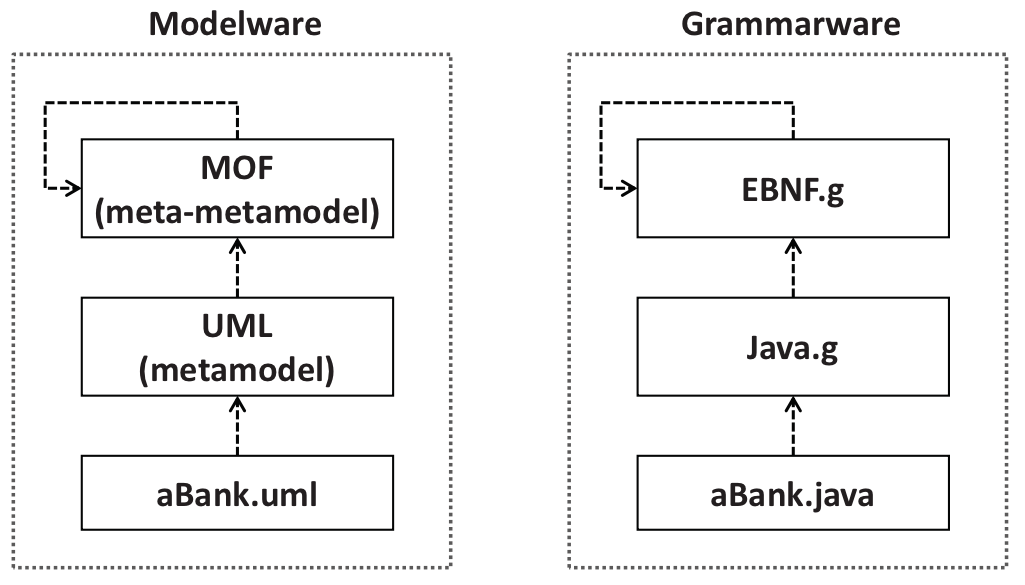
\includegraphics[scale=0.25]{figuras/modelWareVSGrammarWare}
\caption{Modelwarevs.Grammarware.}
\label{fig:modelWareVsGrammarWare}
\end{figure}

MDD é ainda considerado um paradigma atual no contexto de Engenharia de Software. MDD foi popularizado pela \textit{Object Management Group} (OMG) como \textit{Model Driven Architecture} (MDA)~\citep{Kleppe:2003}. Hoje em dia o Eclipse, o qual é um \textit{Integrated Development Environment}, é o ambiente padrão para MDD uma vez que o mesmo contêm uma implementação de referência do MOF, nomeado \textit{Eclipse Modeling Framework} (EMF).

\subsection{\textit{Model-Driven Reverse Engineering} (MDRE)}\label{sec:model_driven_reverse_engineering}

A utilização de MDD no contexto da ER (ou seja, MDRE) é um campo relativamente recente~\citep{Model_Driven_Reverse_Engineering}. No início, os modelos eram apenas utilizados, principalmente, para especificar os sistemas antes da sua implementação (durante a Engenharia Avante). MDRE propõe que modelos não sejam apenas artefatos que ``guiam'' o engenheiro durante tarefas de desenvolvimento e manutenção de software, mas como parte integrante do software~\citep{ThomasMDD}.


Devido ao grande interesse em MDRE, a OMG em 2003 inicio uma força tarefa (ADM \textit{taskforce}) que tinha como intuito padronizar o processo de engenharia reversa. Da mesma forma que MDA, a OMG criou a \textit{Architecture-Driven Mordernization} (ADM) que tem como objetivo criar especificações/padronizações para auxiliar processo de modernização de sistemas legados por meio de um conjunto de metamodelos padronizados. O fluxo de um processo de MDRE apoiada pela ADM possui três fases e é semelhante ao contorno de uma ferradura, são elas: Engenharia Reversa (ER) (do inglês, \textit{Reverse Engineering}), Reestruturação (do inglês, \textit{Restructuring}) e Engenharia Avante (EA) (do inglês, \textit{Forward Engineering}), como pode ser visto na Figura~\ref{fig:ADM_horse_shoes}. Partindo do lado inferior esquerdo, na parte da ER, o conhecimento é extraído do sistema legado e um modelo \textit{Plataform Specific Model} (PDM) é gerado. O modelo PSM serve como base para a geração de um modelo \textit{Platform Independent Model}, ou seja, durante a fase de ER, transformações são feitas como o intuito de se obter uma representação de alto nível do software, independentemente da plataforma utilizada anteriormente.

\begin{figure}[!ht]
\centering
  % Requires \usepackage{graphicx}
  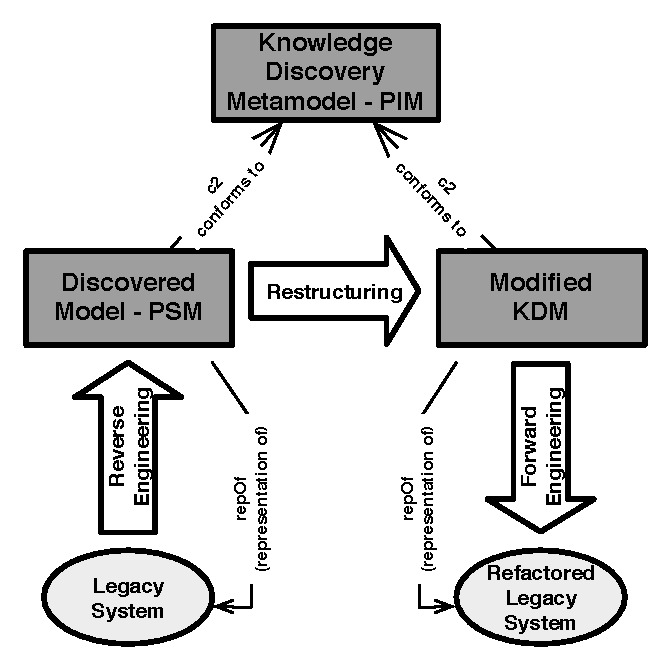
\includegraphics[scale=0.65]{figuras/horseShoe}
\caption{Fluxo do processo de modernização apoiada pela ADM (Adaptada~\citep{OMGADM})}
\label{fig:ADM_horse_shoes}
\end{figure}

O modelo PSM é um modelo especifico de uma plataforma, ou seja, nele existem metadados relacionados a uma plataforma ou linguagem de programação especifica. O modelo PIM é um modelo de abstração mais alto, pois não contém informações especificas de uma determinada plataforma ou linguagem.

Na fase de reestruturação, refatorações, melhorias e novas regras de negócios podem ser introduzidas no sistema, e, com uma representação independente de plataforma do software modernizado, segue-se para a fase de Engenharia Avante. Nessa ultima fase, os modelos são novamente submetidos a uma série de transformações para chegar ao nível de artefatos executáveis, ou seja, código-fonte.

No contexto da ADM, para dar suporte ao processo de modernização independentemente de plataforma e linguagem (PIM), foi criado um metamodelo que possibilita a comunicação entre diferentes plataformas e linguagens, e foi denominado pela ADM \textit{taskforce} de \textit{Knowledge Discovery Metamodel} (KDM)~\citep{ISOKDM}. O KDM provê representações para os sistemas de software existentes em diferentes camadas de abstrações. Cada modelo é representado por um conjunto de visões arquiteturais, ou seja, modelos KDM representando diferentes perspectivas de conhecimento sobre os artefatos dos sistemas de software existentes. Esses modelos são criados automaticamente, semi-automaticamente ou manualmente por meio da aplicação de várias técnicas de extrações de conhecimento, de análises e de transformações.~\citep{PerezCastillo:2011jo}.

O KDM representa artefatos físicos e lógicos de software dos sistemas legados em diferentes níveis de abstração e constitui dozes pacotes organizados em quatro camadas, são elas: infraestrutura (\textit{infrastructure}), elementos de programa (\textit{program elements}), recursos de tempo de execução (\textit{runtime resources}) e abstração (\textit{abstractions})~\citep{PerezCastillo:2011jo}. Na Figura~\ref{fig:KDMArchitecture} está representada a arquitetura do KDM ilustrando a forma como as camadas se relacionam, quais são os pacotes pertencentes a cada camada e a separação dos seus interesses. Cada camada baseia-se na camada anterior, dessa forma, elas estão organizadas em pacotes que definem um conjunto de elementos do metamodelo, cujo propósito é representar um interesse específico e independente do conhecimento relacionado a sistemas legados.

\begin{figure}[!ht]
\centering
  % Requires \usepackage{graphicx}
  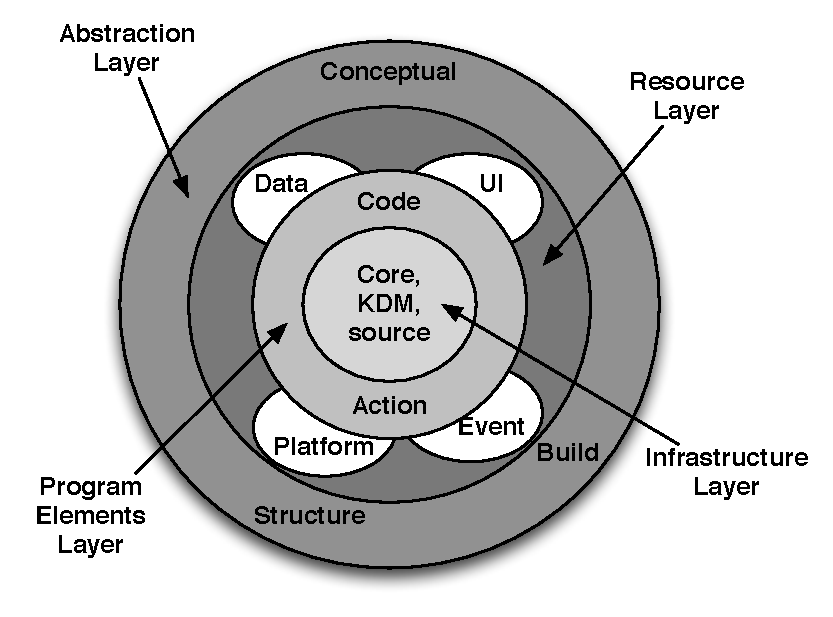
\includegraphics[scale=0.65]{figuras/Layers_packages_and_separations_of_concerns_in_KDM}
\caption{Arquitetura do KDM (adaptada~\citep{OMGADM})}
\label{fig:KDMArchitecture}
\end{figure}

Três pacotes importantes do KDM no contexto deste trabalho são: (\textit{i}) pacote \textit{Code}, (\textit{ii}) \textit{Action} e (\textit{iii}) \textit{Structure}. Os dois primeiros pacotes contêm metaclasses para representar elementos de programação, tais como, classes, métodos, atributos, etc. Dessa forma, utilizando esses dois pacotes foi possível criar/adaptar um catalogo de refatoração para o contexto do KDM. Assim, todos as refatorações que foram adaptadas para o KDM agora são independentes de linguagem e plataforma. O terceiro pacote por sua vez (\textit{Structure}), define elementos de metamodelo que representam componentes de arquitetura de sistemas de software existentes. Por exemplo, esse pacote define as seguintes metaclasses: \textit{Subsystem}, \textit{Component}, \textit{Layer}, \textit{SoftwareSystem}, \textit{ArchitectureView}. Ressalta-se ainda que esse ultimo pacote, é de suma importância para as próximas atividades do outorgado, uma vez que verificação de conformidade nível arquitetural serão implementadas para o KDM. Além disso, também serão definidas refatorações em nível arquitetural.

\subsection{Apoio ferramental}\label{sec:apoio_ferramental}

Diversas ferramentas de modelagem estão disponíveis para o desenvolvimento empresarial baseado em modelo, uma plataforma de ferramentas que se tornou proeminente no mundo da MDRE é o IDE Eclipse. Um conjunto de ferramentas interessantes para MDRE foram disponibilizados para essa IDE, permitindo, assim diversas iniciativas sobre esta plataforma. No contexto, do projeto em questão algumas iniciativas foram utilizadas: (\textit{i}) \textit{Eclipse Modeling Framework} (EMF), (\textit{ii}) Xtext, (\textit{iii}) Acceleo e (\textit{iv}) \textit{ATL Transformation Language} (ATL). 

\textit{Eclipse Modeling Framework} (EMF) é a principal iniciativa do IDE Eclipse no contexto de MDRE por várias razões. Primeiro, EMF permite a definição de metamodelos tendo como base uma linguagem de metamodelagem denominada Ecore. Em segundo lugar, EMF fornece um gerador de metamodelos, ou seja, uma API baseada em Java para manipulação de modelos. Em terceiro lugar, EMF contêm uma poderoso API que abrangem diferentes aspectos, tais como a serialização e deserialização de modelos de/para \textit{XML Metadata Interchange} (XMI). Xtext é um framework para desenvolvimento de Linguagens Específicas de Domínio (do inglês, \textit{Domain-Specific Language}). Acceleo é uma implementação pragmática do OMG para fornecer suporte a transformações \textit{Model2Text}. Por fim, ATL é uma linguagem de transformação de modelos, ou seja provê suporte a transformações \textit{Model2Model}. 











		\subsection{Resumo do Plano Inicial}\label{resumo_plano_inicial}
			\input{text/resumo_do_palno_inicial}

\section{Cronograma e Resumo das Atividades Realizadas no Período}\label{cronograma}
A seguir é apresentado uma \textit{timeline} que descreve todas as atividades realizadas durante o período de vigência e que serão realizadas o período pelo bolsista para o desenvolvimento deste projeto. Em seguida, é apresentada uma descrição de cada evento presente na \textit{timeline}. Ressalta-se que todos os artigos que foram publicados durante o período de vigência desse relatório estão destacados tanto na \textit{timeline} quanto na descrição pelo símbolo $\Rightarrow$ ou $\Leftrightarrow$. $\Leftrightarrow$ ilustra capítulo de livro, enquanto o símbolo $\Rightarrow$ refere-se a conferências. Além disso, vale destacar que maiores informações sobre cada evento serão descritas nas seções seguintes.

\begin{itemize}

\item \textbf{Mar 6, 2013 - Jan 20, 2015} - Estudo detalhado sobre ADM e KDM;
\item \textbf{Mar 9, 2013 - Dec 5, 2013} - Implementação de um catalogo de refatoração para o KDM;
\item \textbf{Apr 6, 2013 - Mar 20, 2014} - Realização do Doutorado Sanduíche no INRIA, Lille, França;
\item \textbf{Nov 6, 2013 - Oct 23, 2014} - Elaboração de um metamodelo de refatoração;
\item $\Rightarrow$ Artigo 1 - Concern-Based Refactorings Supported by Class Models to Reengineer Object-Oriented Software into Aspect-Oriented Ones;
\item $\Rightarrow$ Artigo 2 - F3: From features to frameworks;
\item $\Rightarrow$ Artigo 3 - An Approach to Develop Frameworks from Feature Models;
\item $\Rightarrow$ Artigo 4 - F3T: From Features to Frameworks Tool;
\item $\Rightarrow$ Artigo 5 - CCKDM - A Concern Mining Tool for Assisting in the Architecture-Driven Modernization Process;
\item $\Rightarrow$ Artigo 6 - A Combined Approach for Concern Identification in KDM models;
\item $\Leftrightarrow$ Artigo 7 - Developing Frameworks from Extended Feature Models;
\item $\Rightarrow$ Artigo 8 - Evaluating the Effort for Modularizing Multiple-Domain Frameworks towards Framework Product Lines with Aspect-Oriented Programming and Model-Driven Development;
\item $\Rightarrow$ Artigo 9 - Data Network in Development of 3D Collaborative Virtual Environments: A Systematic Review;
\item $\Rightarrow$ Artigo 10 - Towards a Refactoring Catalogue for Knowledge Discovery Metamodel;
\item $\Rightarrow$ Artigo 11 - A Mapping Study on Architecture-Driven Modernization;
\item $\Rightarrow$ Artigo 12 - KDM-AO: An Aspect-Oriented Extension of the Knowledge Discovery Metamodel;
\item $\Rightarrow$ Artigo 13 - Investigating Lightweight and Heavyweight KDM Extensions for Aspect-Oriented Modernization;
\item $\Rightarrow$ Artigo 14 - KDM-RE: A Model-Driven Refactoring Tool for KDM;

\item \textbf{16/2/2015 - 19/2/2016} - Esse período representa as Etapas Seguintes;

\begin{itemize}
	\item \textbf{7/3/2015 - 8/7/2015} - Elaboração de Artigos;
	\item \textbf{15/5/2015 - 28/11/2015} - Implementar Refatorações Arquiteturais;
	\item \textbf{28/5/2015 - 30/09/2015} - Estudo Experimental;
	\item \textbf{29/06/2015 - 3/11/2015} - Redação da Tese;
	\item \textbf{08/09/2015 - 10/01/2016} - Evolução Ferramental;
	\item \textbf{Fevereiro} - Defesa do Doutorado;
\end{itemize}

\end{itemize}


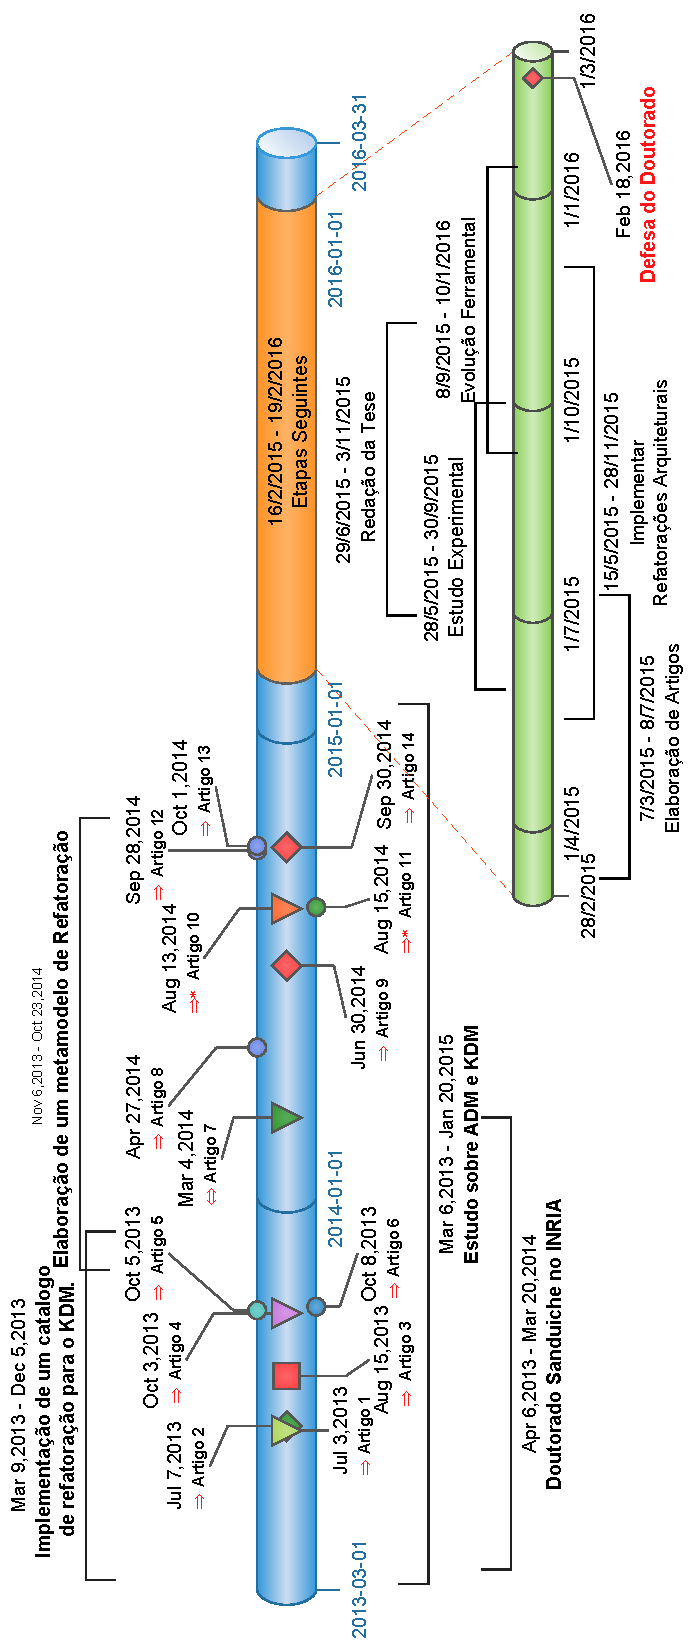
\includepdf[pages={-}]{figuras/timeLine}

%\subsection{Resumo das Atividades Realizadas no Período}\label{atividades_realizadas}

 	\subsection{Estágio no Exterior}

O estágio contou com o apoio financeiro da CNPQ (Processo: 241028/2012-4) e foi realizado no \textit{Institut national de recherche en informatique et en automatique} (INRIA), França. O aluno ficou na França por um ano (Abril de 2013 - Abril de 2014) sob a supervisão do professor Doutor Nicolas Anquetil. O grupo de pesquisa é especializado em remodularização e modernização de sistemas orientados a objetos com enfoque em \textit{Model-Driven Development}. 

Dois projetos foram conduzidos durante a estadia na França, descritos nas Seções X e Y. É importante enfatizar que ambos os projetos são diretamente relacionados à realização deste projeto de doutorado.

O vínculo com o CNPQ foi encerrado no mês de Abril e a bolsa da FAPESP foi reatividade. Uma cópia do parecer emitido pelo orientador no exterior pode ser encontrado no Apêndice A.

\subsection{Mapeamento Sistemático}

Quando se conduz uma revisão de literatura sem o pré-estabelecimento de um protocolo de revisão há um direcionamento por interesses pessoais, o que leva a resultados pouco confiáveis. Neste contexto, pesquisadores vem utilizando uma técnica denominada de Mapeamento Sistemático (MS) para auxiliar o pesquisador a conduzir um revisão bibliográfica de forma totalmente sistemática com o intuito de evitar que trabalhos importantes fiquem fora de suas pesquisas. Um MS é caracterizada por ser um meio de avaliar e interpretar todas as pesquisas disponíveis, referentes a um questão de pesquisa, tema, área ou fenômeno de interesse. O MS tem como objetivo apresentar uma avaliação justa de um tema de pesquisa, utilizando uma metodologia confiável, rigorosa e auditável~\cite{kit04}.

De acordo com~\citet{kit04} o MS implica na forma mais adequada para se identificar, avaliar e interpretar toda pesquisa importante para um tema em particular. Resume-se que um MS configura um alicerce para novas atividades de pesquisa acerca de determinado tema. Dessa forma, foi realizado um MS sobre \textit{Architecture-Driven Modernization} (ADM) e \textit{Knowledge-Discovery Metamodel} (KDM). A nossa motivação para realizar esse MS é identificar os temas que têm sido mais investigados, bem como os temas que ainda não foram investigados. Embora, a ADM é uma abordagem relativamente nova, OMG afirma que ela é uma importante abordagem pois combina dois dos principais campos da Engenharia de Software, ou seja, \textit{Model-Driven Development} e Engenharia Reversa. Desde a definição da ADM muitos esforços têm enfatizado a modernização de sistemas legados por meio desta abordagem. Neste contexto, é importante realizar uma investigação mais sistemática dos temas englobados por esta área de pesquisa. 

Para atingir este objetivo, foi realizado um MS. Os resultados, bem como o protocolo de pesquisa elaborado, foram publicados no \textit{IEEE Information Reuse and Integration} (IRI 2014) , o qual tem qualis B2. O artigo foi apresentado pelo bolsista em Agosto de 2014 em São Francisco, California. Maiores detalhes sobre esse artigo pode ser obtido no Apêndice A deste relatório. O mesmo anexo contem uma cópia da obra submetida.


\subsection{Estabelecimento do Catalogo de Refatoração para o metamodelo KDM} % (fold)
	 \label{sub:catalogo_kdm}

Foi elaborado um catalogo dedicado para ser aplicado no metamodelo do KDM. Mais especificamente esse catalogo foi adaptado com base em catálogos já disponíveis na literatura. Para a definição desse catalogo de refatoração, foi utilizado um formato inspirado pelo~\cite{refactImpro}. Em outras palavras, o catalogo foi descrito da seguinte forma: (\textit{i}) o nome do refatoração, (\textit{ii}) descrição da típica situação onde a refatoração deve ser aplicada, (\textit{iii}) descrição da solução para solucionar uma determinada situação problemática, (\textit{iv}) pre-condições que devem ser satisfeitas para aplicar a refatoração, (\textit{v}) os parâmetros necessários para executar a refatoração e (\textit{vi}) descrição dos passos para realizar a refatoração.

O catalogo de refatoração é estruturado em quatro grupos como pode ser observado na Tabela~\ref{tab:catalogue}, a qual contêm 17 refatorações. O primeiro grupo chamada \textit{Rename Feature} consiste de refatorações para renomear \textit{ClassUnit}, \textit{StorableUnits} e \textit{MethodUnits}. O segundo grupo, \textit{Moving Features Between Objects} consiste de refatorações simples, tais como mover ou criar características, ou seja, criar ou mover atributos, métodos ou classes. O terceiro grupo,  \textit{Organizing Data}, é responsável por definir um conjunto de refatorações para ser organizar a estrutura do código-fonte. Por fim, o quatro grupo, \textit{Dealing With Generalization}, representa refatorações para mover métodos e/ou atributos sobre uma especifica hierarquia de classes. 

\begin{table}[!h]
\caption{Refactorings Adapted to KDM}
\label{tab:adaptedRefactoring}
\centering
  % Requires \usepackage{graphicx}
  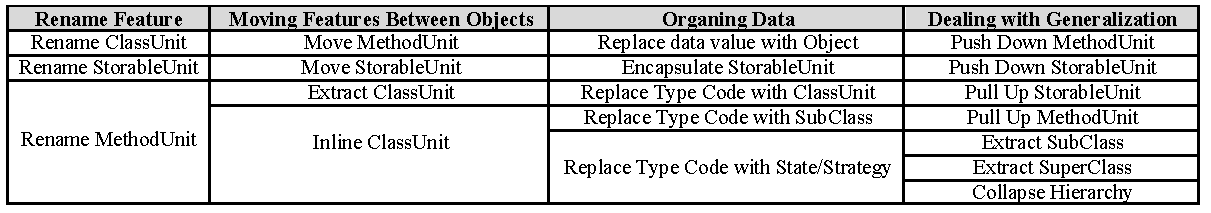
\includegraphics[scale=0.67]{figuras/NovoCatalogue}
\end{table}

Vale ressaltar que um artigo descrevendo o catalogo de refatoração adaptado para o KDM também foi no \textit{IEEE Information Reuse and Integration} (IRI 2014) , o qual tem qualis B2. O artigo foi apresentado pelo bolsista em Agosto de 2014 em São Francisco, California. Além disso, o bolsista participou das sessões técnicas e palestras. Maiores detalhes sobre esse artigo pode ser obtido no Apêndice B deste relatório. O mesmo contem uma cópia da obra submetida.

\subsection{Um ambiente integrado para desenvolvimento e apoio para o catalogo de refatorações do metamodelo KDM}

Durante a revisão sistemática pode-se averiguar que tanto o processo ADM e o seu metamodelo KDM têm sido vastamente utilizado na literatura para auxiliar a modernização de sistemas legados. No entanto, também pode-se verificar qua até o momento não existe nenhum ambiente integrado de desenvolvimento para guiar o engenheiro para automaticamente aplicar as refatorações e modernizações como existe em outros paradigmas, tais como o paradigma orientado a objetos. Para mitigar tal limitação, durante o período de vigência da bolsa foi desenvolvido um \textit{plug-in} utilizando a plataforma do Eclipse. 

Esse \textit{plug-in} fornece um ambiente para realizar as refatorações apresentadas na Seção~\ref{sub:catalogo_kdm} de forma totalmente automatizada. Na Figura~\ref{fig:ferramenta} é ilustrado todo o processo no qual o \textit{plug-in} é baseado. Como pode ser observado nessa figura a utilização do \textit{plug-in} pode ser ilustrada em três passos: (\textit{i}) engenharia reversa (\textit{reverse engineering}), (\textit{ii}) refatorações (\textit{refactorings}) e (\textit{iii}) engenharia avante (\textit{forward engineering}). Maiores detalhes sobre tais passos são descritos nas próximas seções.

\begin{figure}[!h]
 \centering
 \scalebox{0.6}{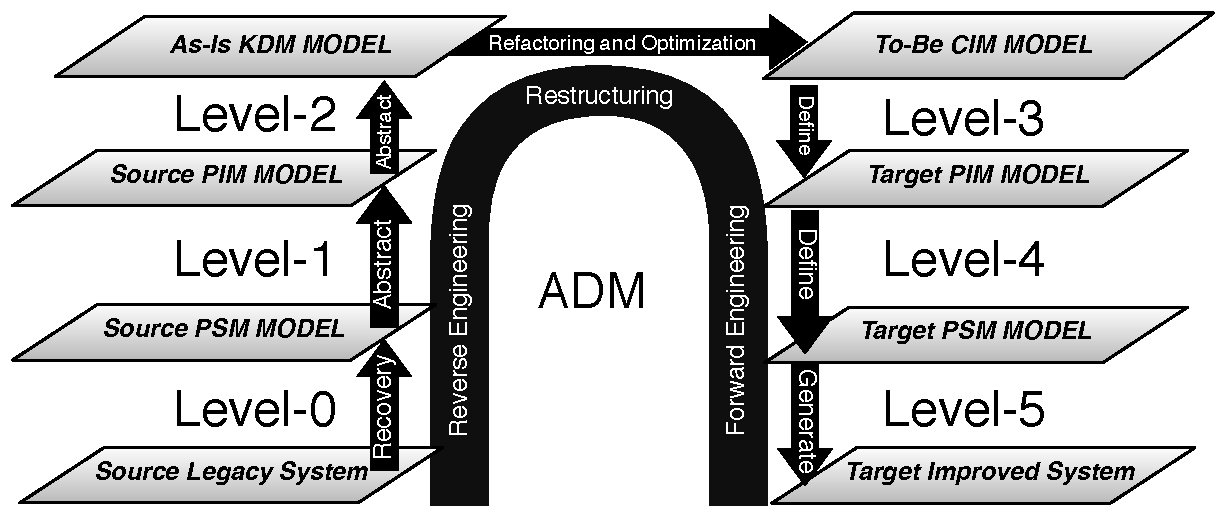
\includegraphics{figuras/processoDaFerramenta}}

\caption{Passos para utilização do \textit{plug-in}}
 \label{fig:ferramenta}
\end{figure}


 \subsubsection{Engenharia Reversa}

Para iniciar esse passo o engenheiro de software deve entrar com um arquivo que representa uma instância do metamodelo KDM ou um determinado código-fonte para realizar a refatoração. No caso do código-fonte ser a entrada escolhida, o engenheiro de software começa o processo no \textbf{Level-0} escolhendo um projeto no Eclipse\footnote{https://www.eclipse.org/} que contenha o código-fonte para realizar as refatorações. Posteriormente, no \textbf{Level-1} o código-fonte precisa ser transformado para um modelo especifico de plataforma (no inglês - Platform-Specific Model (PSM)). Esse PSM representa uma instância do código-fonte em um nível mais abstrato do código-fonte. Para realizar essa transformação (código-fonte para PSM) foi implementado um extrator de modelo em Java.

Após criar o PSM o próximo level (\textbf{Level-2}) consiste em transformar o PSM para um Modelo Independente de plataforma (no inglês - Platform-Indented Model (PIM)) o qual é baseado no metamodelo do KDM. Nesse level o \textit{plug-in} utiliza o \textit{framework} MoDisco\footnote{http://www.eclipse.org/MoDisco/} para realizar a transformação de PSM para PIM.

Na Figura~\ref{fig:plugin} é apresentado uma visão geral do \textit{plug-in} desenvolvido pelo bolsista durante a período de vigência da bolsa. Apenas para o propósito de explicação, foi identificado quatro principais regiões do \textit{plug-in}, veja Figura\ref{fig:plugin} \textcircled{a}, \textcircled{b}, \textcircled{c} and \textcircled{d}.

\begin{figure}[!h]
 \centering
 \scalebox{0.9}{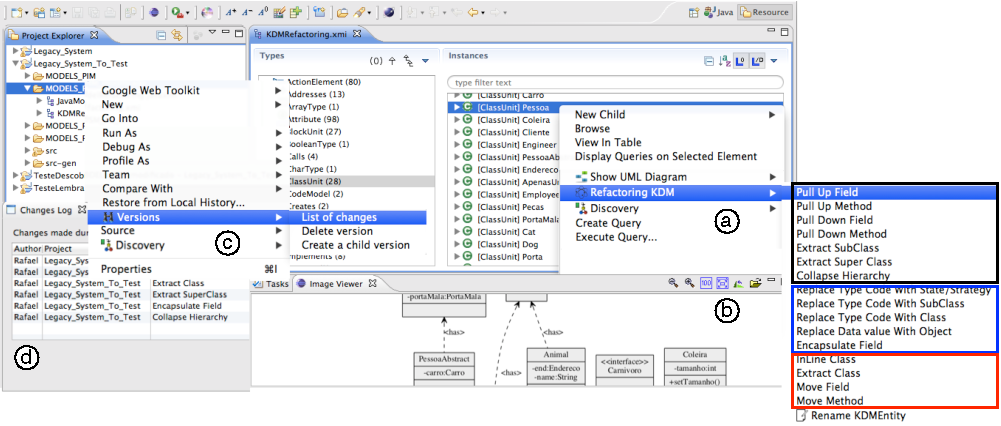
\includegraphics{figuras/ScreenShot_tool}}
\caption{Visão geral do \textit{plug-in} desenvolvido}
 \label{fig:plugin}
\end{figure}

Como já salientado anteriormente todas as refatorações fornecidas pelo \textit{plug-in} são feitas com base no metamodelo KDM. Dessa forma, para auxiliar o engenheiro de software a realizar as refatorações um menu chamado \textit{Refactoring KDM} foi adicionado, veja Figura~\ref{fig:plugin}\textcircled{a}. Utilizando esse menu o engenheiro de software pode interagir com o metamodelo do KDM e escolher qual refatoração deve ser executada. Note que na região \textcircled{a} da Figura~\ref{fig:plugin} é possível ver todas as 17 refatorações implementadas no \textit{plug-in}.

Na região \textcircled{b} da Figura~\ref{fig:plugin} é apresentado um diagrama de classe. Esse diagrama pode ser utilizado pelo engenheiro de software antes ou depois de aplicar as refatorações no modelo KDM. Usualmente o engenheiro pode utilizar esse diagrama antes de aplicar refatorações para decidir onde deve-se realmente aplicar as refatorações. Além disso, esse diagrama é útil por que geralmente sistemas legados não contêm nenhum tipo de documentação, sendo o código-fonte o único artefato disponível do mesmo. Portanto, criar um diagrama de classe durante a execução de refatorações no sistema legado pode ser uma boa alternativa para melhorar a documentação de um determinado sistema.

O \textit{plug-in} também fornece múltiplas versões de um sistema em nível de modelos, ou seja, em nível de modelos KDM. O objetivo é permitir que o engenheiro de software trabalhe interativamente em vários modelos, permitindo assim que o engenheiro de software escolha e explore diferentes caminhos de refatoração. Como pode ser observado na região  \textcircled{c} da Figura~\ref{fig:plugin}, o engenheiro deve selecionar o arquivo KDM e escolher a opção ``\textit{Versions}''. Três opções são disponíveis nesse menu (\textit{i}) \textit{List of Changes}, (\textit{ii}) \textit{Delete version} and (\textit{iii}) \textit{Create a child version}. A primeira opção mostra todas refatorações que já foram feitas pelo engenheiro (ver região \textcircled{d} ) - a segunda opção é responsável por deletar uma versão - e a ultima opção criar uma cópia do arquivo KDM, permitindo assim que o engenheiro aplique outras refatorações e explore diferentes caminhos de refatoração sem afetar o modelo KDM principal do projeto.


 \subsubsection{Executando Refatorações no \textit{Plug-in}}

Após o engenheiro clicar no menu da região \textcircled{a} (ver Figura~\ref{fig:plugin}) e escolher qual refatoração aplicar um \textit{Wizard} será mostrado. Para explicação, considere que o engenheiro de software escolheu aplicar a refatoração denominada \textit{Extract Class}. Então o engenheiro deve selecionar qual metaclass o mesmo deseja extrair, esse passo é ilustrado na Figura~\ref{fig:wizard} (a). Posteriormente o \textit{plug-in} executa o \textit{Wizard} como ilustrado na Figura~\ref{fig:wizard} (b). Como pode ser observado, aqui o engenheiro de software pode atribuir um nome para a nova metaclasse. Além disso, uma prévia de todos os detectados \textit{StorableUnits} e \textit{MethodUnis} que podem ser extraídos e adicionados na outra classe também são mostrados. O engenheiro pode também selecionar se a nova classe será uma classe interna ou uma classe normal. Também é possível especificar se métodos assessores (\textit{getters} e \textit{setters}) devem ser criados ou não. 

\begin{figure}[!h]
 \centering
 \scalebox{0.6}{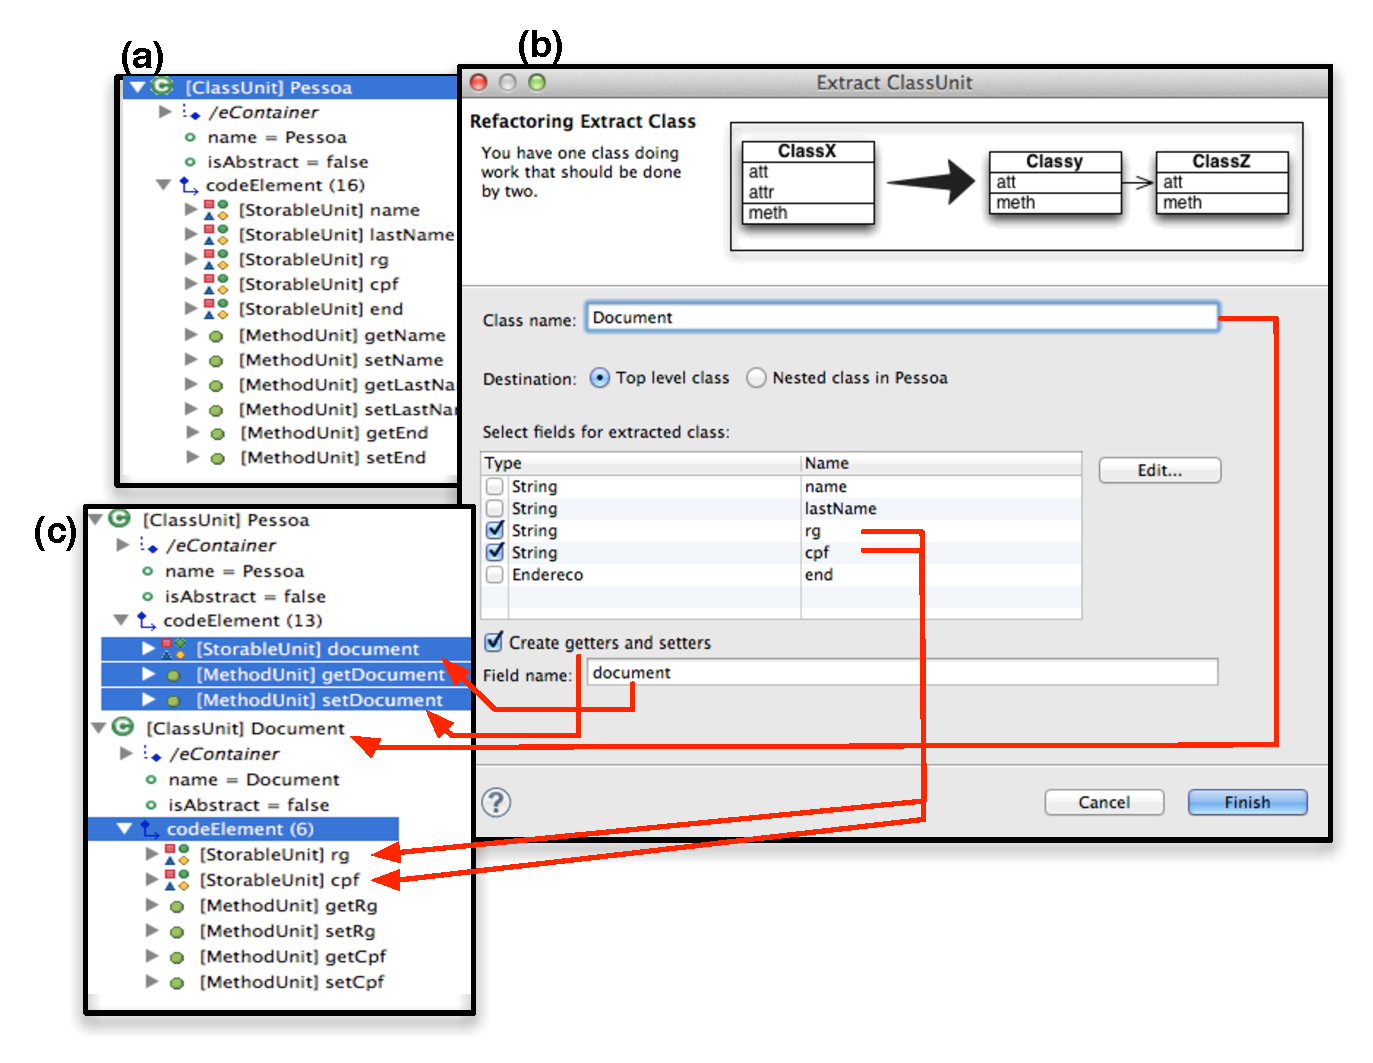
\includegraphics{figuras/Wizard2}}
\caption{Extract Class Wizard}
 \label{fig:wizard}
\end{figure}

Após o engenheiro preencher todos os campos necessários, ele pode clicar no botão \textit{Finish} e então a refatoração \textit{Extract Class} é executada. Como pode ser observado na Figura~\ref{fig:wizard} (c) uma nova instância de \textit{ClassUnit} denominada \textit{Document} foi criada - dois \textit{StorableUnits} da metaclasse \textit{Pessoa}, ``rg'' e ``CPF'' foram movidas para \textit{Document}.


 \subsubsection{Engenharia Avante}

Após o engenheiro realizar todas as refatorações no KDM os próximos passos são: (\textit{i}) transformar o KDM para um PSM e (\textit{ii}) transformar o PSM para artefatos físicos (código-fonte). O primeiro passo é executado baseado em um conjunto de transformações utilizando a linguagem ATL Transformation Languag (ATL)\footnote{https://www.eclipse.org/atl/}. O último passo consiste em utilizar \textit{templates} para gerar o código-fonte refatorado.  Na Figura~\ref{fig:forward} é apresentado como é feita a geração de código-fonte.

\begin{figure}[!h]
 \centering
 \scalebox{0.4}{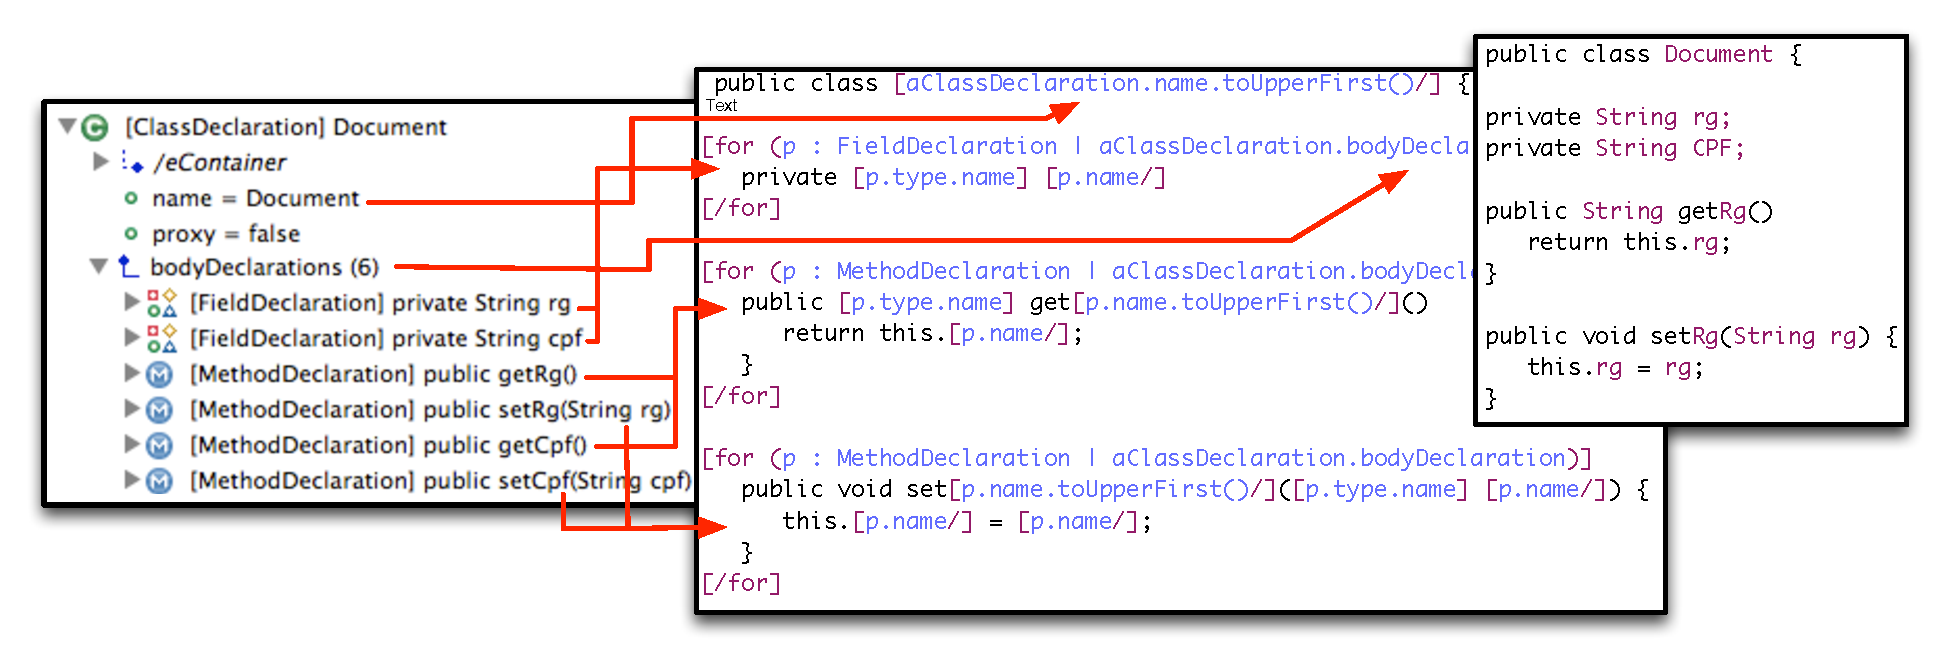
\includegraphics{figuras/ForwardEngineering}}
\caption{Passos da Engenharia Avante}
 \label{fig:forward}
\end{figure}

 \subsubsection{Arquitetura do \textit{plugin}}

Na Figura~\ref{fig:architecture} é ilustrado a arquitetura do \textit{plug-in} desenvolvido durante o período de vigência da bolsa. Como pode ser observado nessa figura, a primeira camada (\textit{layer}) é o \textit{Core Framework}. Essa camada representa que o \textit{plug-in} foi desenvolvida utilizando como base a plataforma de desenvolvimento Eclipse. Além disso, nessa camada pode-se observar que também foi utilizado Java e Groovy como linguagem de programação. Também é possível identificar que nessa camada alguns \textit{plug-ins} da plataforma de desenvolvimento Eclipse foram utilizados, tais como MoDisco\footnote{http://www.eclipse.org/MoDisco/} e EMF\footnote{https://www.eclipse.org/modeling/emf/}. Modisco e EMF ambos foram utilizados pois fornecem uma \textit{Application Programming Interface} (API) para facilitar o acesso ao metamodelo KDM.

\begin{figure}[!h]
 \centering
 \scalebox{0.8}{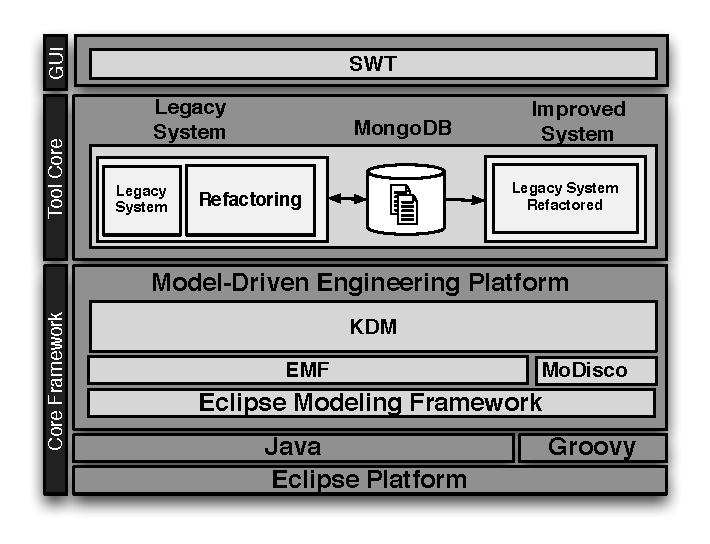
\includegraphics{figuras/Arquitetura}}
\caption{Arquitetura do \textit{plug-in}}
 \label{fig:architecture}
\end{figure}

A segunda camada, \textit{Tool Core}, é onde todas as refatorações fornecidas pelo \textit{plug-in} foram implementadas. A ultima camada é onde a interface gráfica do \textit{plug-in} foi desenvolvida. Vale ressaltar que um artigo sobre esse \textit{plugin} foi publicado no  2nd \textit{Workshop on Software Visualization, Evolution and Maintenance} (VEM). O bolsista esteve presente nesse evento, apresentado o artigo e participando das sessões técnicas e palestras. Mais detalhes sobre este \textit{plugin} podem ser encontrados na cópia desse artigo no Apêndice C.

\subsection{Um Metamodelo para Especificar Refatorações para o KDM}

Durante o desenvolvimento e evolução de software novas funcionalidades geralmente são adicionadas ou são ajustadas a novas exigências. Devido a tais alterações, a flexibilidade da arquitetura desse sistema pode ser um fator desafiador. Em outros casos, após aplicar um conjunto de alterações a arquitetura continua perfeitamente adequada. Porém, usualmente é necessário aplicar mudanças na arquitetura dessa sistema para confortar tais alterações. 

Para melhorar o projeto de um determinado software, geralmente os engenheiros de software gastam uma quantidade significativa de tempo reestruturando o software manualmente. No entanto, reestruturar código manualmente além de ser uma tarefa que demanda tempo é totalmente propicia a erros. Não importa a atenção dispendida pelo engenheiro de software durante a atividade de reestruturação, se o sistema é relativamente grande, há uma boa chance de que o mesmo irá ter o seu comportamento alterado após tal atividade. Como ressaltado anteriormente é de suma importância que o comportamento do sistema seja preservado após a reestruturação, assim, o conceito de refatoração deve ser aplicado (ver Seção~\ref{sub:refatoracao}).

 Hoje em dia refatoração é utilizada tanto no âmbito acadêmico quanto na industria. Refatoração é uma área muito madura e muito difundida. Além disso, várias IDEs executam facilmente e de forma segura um conjunto refatorações para um vasto número de linguagens de programação. Com o surgimento de MDD é importante que os conceitos de refatorações sejam adaptados tanto para MDRE (ver Seção~\ref{sec:model_driven_reverse_engineering}) e ADM. Uma iniciativa têm sido conduzida pelo outorgado. Mais especificadamente o bolsista definiu um ambiente integrado para desenvolvimento e apoio para o catalogo de refatorações do metamodelo KDM~\citep{KDM_RE_A_Model_Driven_Refactoring_Tool_for_KDM}. Maiores informações podem ser obtidas no artigo publicado, o mesmo pode ser visualizado na integra no Apêndice X.

Um olhar mais atento à reutilização de refatorações levanta a questão sobre o que pode ser reutilizado e o que não pode. Trabalhos anteriores nesta área tem mostrado que há potencial para reutilização, mas é limitado, de uma forma ou de outra. No entanto, pesquisas também apontam que algumas características não podem ser capturadas na parte reutilizável de uma refatoração. Por exemplo, uma refatoração genérica não pode fazer suposições sobre a semântica de uma linguagem de programação. 

Embora a ADM e, principalmente o KDM, tenham sido propostos para apoiar a modernização de sistemas legados, até o momento não existem propostas de um metamodelo para especificar refatorações para o KDM. Portanto, os engenheiros de modernização precisam desenvolver suas próprias soluções para transformar instâncias KDM origem em alvo. Durante o mapeamento sistemático conduzido e publicado pelo outorgado~\citep{iri_systematic_mapping_ADM_2014} (ver Apêndice X) pôde-se observar na literatura a carência de estudos que definem um metamodelo para especificar refatorações para KDM. Sem a adequada representação de refatorações no KDM, a realização de uma refatoração pode se tornar propensa a erros. Assim, é de suma importância definir uma extensão para o KDM em que os engenheiros de modernização possam especificar refatorações independentes de plataforma.

Como já ressaltado existe uma forte necessidade de reutilizar refatorações no contexto da ADM e, principalmente para o metamodelo KDM. Para permitir tal reutilização, as partes de refatorações que podem ser generalizadas devem ser separadas das que são específicas. Por exemplo, considere a refatoração \textit{RenameElement}. As etapas necessárias para executar tal refatoração são iguais, não importa que tipo de elemento precisa ser renomeado. Por exemplo, depois de alterar o valor de um atributo do tipo \textit{String}, todas as referências daquele elemento precisa também ser atualizado. O atributo concreto pode variar dependendo da linguagem de programação, mas o procedimento é o mesmo.	

Com base no exemplo anterior é possível identificar algumas idéias iniciais. Na Figura~\ref{fig:processoDOMETAMODELO} é ilustrado os principais conceitos que foram utilizados para criar o metamodelo de refatoração para o KDM. Em primeiro lugar, as partes estruturais de uma refatoração (classes, métodos, atributos, etc), ou seja, os elementos que são transformados, foram considerados bons candidatos para o reuso (ver Figura~\ref{fig:processoDOMETAMODELO} \ding{182}) e assim utilizados como base para a criação do metamodelo de refatoração. Em segundo lugar, foi possível identificar na literatura pesquisas que executam uma refatoração utilizando um conjunto de composições de transformações por meio de linguagens de transformações, tais como OCL e ATL (ver Figura~\ref{fig:processoDOMETAMODELO} \ding{183}). Além disso, também foi constatado que a grande maioria das refatorações são realizadas utilizando operações primárias, tais como: \textit{add}, \textit{remove}, \textit{move}, \textit{create}, entre outras. Tais operações primárias também foram incluídas no metamodelo de refatoração para o KDM (ver Figura~\ref{fig:processoDOMETAMODELO} \ding{184}). Assim, os engenheiros de modernização podem realizar um \textit{chain of primary operations} permitindo a especificar/criar novas refatorações. O catalogo de refatoração proposto por Fowler~\citep{refactImpro} também foi considerado durante a criação do metamodelo de refatoração para o KDM como pode ser observado na Figura~\ref{fig:processoDOMETAMODELO} \ding{185}.


\begin{figure}[!h]
 \centering
 \scalebox{0.6}{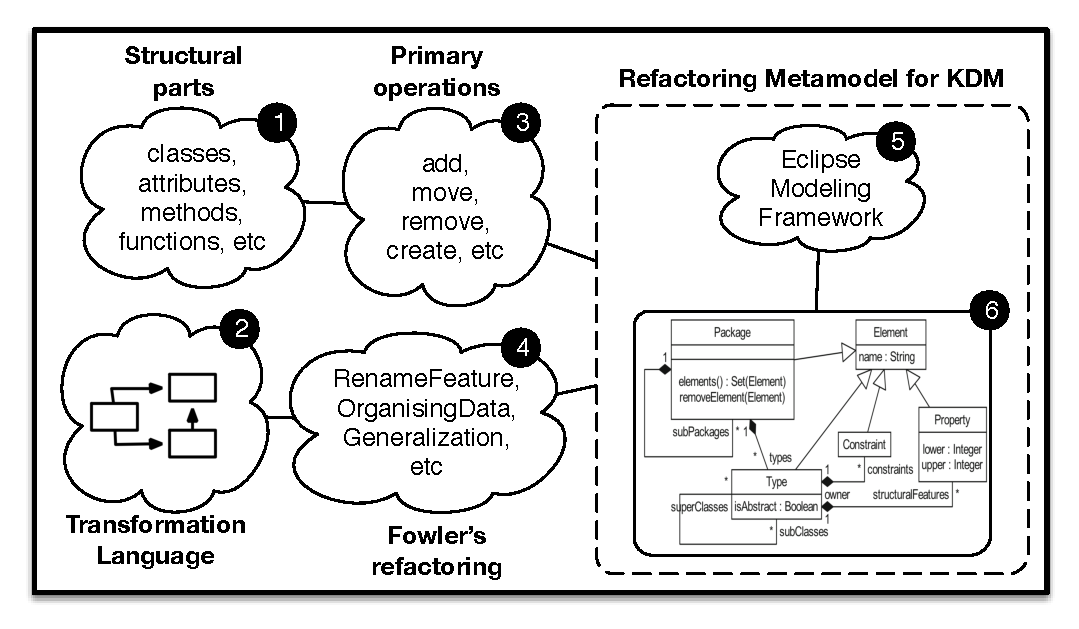
\includegraphics{figuras/ProcessoDOMetamodelo}}
\caption{Princípios e critérios utilizados para criar o metamodelo de refatoração para o KDM}
 \label{fig:processoDOMETAMODELO}
\end{figure}

\begin{figure}[h]
 \centering
 \scalebox{0.6}{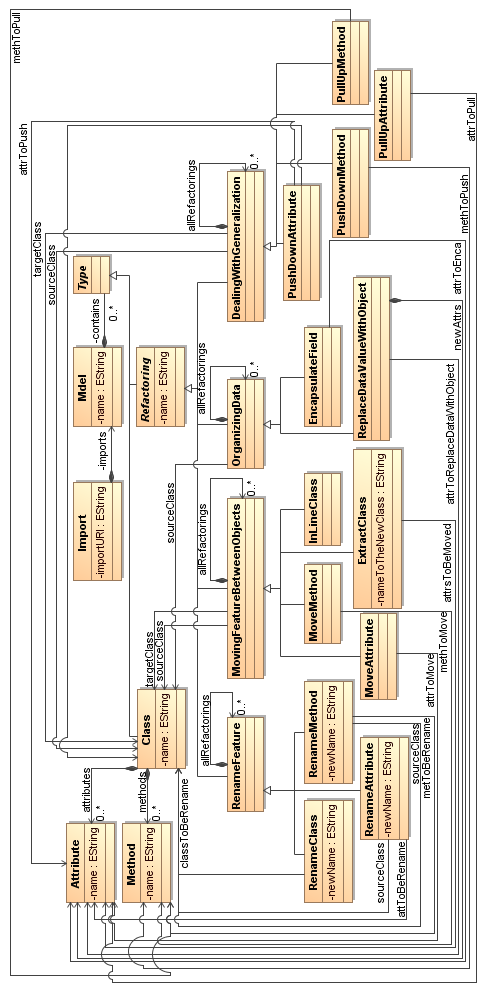
\includegraphics{figuras/metamodelo7}}
\caption{Metamodel de Refatoração para o KDM}
 \label{fig:METAMODELO}
\end{figure}

Para reutilizar a parte estrutural de uma refatoração, um modelo que represente essa estrutura é necessário. Para o exemplo \textit{RenameElement}, a estrutura basicamente consiste de uma \textit{metaclass} em um \textit{metamodel}. Outras refatorações, tais como \textit{ExtractClass} possuem restrições estruturais mais complexas, como a exigência de que a classe que será extraída esteja contida em um \textit{container object}. O metamodelo de refatorações para o KDM foi definido utilizado EMF (Figura~\ref{fig:processoDOMETAMODELO} \ding{186}). O metamodelo pode ser visualizado na Figura~\ref{fig:METAMODELO}. As \textit{metaclasses} que compõem o metamodelo de refatoração para o KDM são definidas da seguinte forma:
 
\begin{itemize}

\item \textit{Refactoring} é o elemento raiz utilizado para armazenar todas as informações sobre as refatorações.

\item \textit{RenameFeature} corresponde às categorias de refatorações relacionadas a ação de renomear.\textit{RenameFeature} também armazena todas as refatorações relacionadas com a ação de renomear utilizando o \textit{metaattribute} \textit{allRefactorings}.

\item \textit{RenameClass} representa uma instância da refatoração \textit{rename Class}.  A semântica para a utilização da \textit{RenameClass} consiste em: (\textit{i}) especificar uma \textit{ClassUnit} (\textit{classToBeRenamed}), (\textit{ii}) bem como uma \textit{string} que representa o novo nome (\textit{newName}) da \textit{ClassUnit} após a aplicação da refatoração \textit{renameClassUnit}.

\item \textit{RenameAttribute} representa uma instância da refatoração \textit{rename Attribute}. A semântica para a utilização da \textit{metaclass} \textit{RenameAttribute} consiste em: (\textit{i}) especificar a \textit{ClassUnit} (\textit{sourceClass}) que armazena todos os atributos e todos os métodos, (\textit{ii}) o atributo que será renomeado (\textit{attToBeRename}) e (\textit{iii}) uma \textit{string} que representa o novo nome (\textit{newName}) do atributo após a aplicação da refatoração \textit{renameAttribute}.

\item \textit{RenameMethod} representa uma instância da refatoração \textit{rename Method}. A semântica para a utilização da \textit{metaclass} \textit{RenameMethod} consiste em: (\textit{i}) especificar a \textit{ClassUnit} (\textit{sourceClass}) que armazena todos os atributos e todos os métodos, (\textit{ii}) o método que será renomeado (\textit{methToBeRename}) e (\textit{iii}) uma \textit{string} que representa o novo nome (\textit{newName}) do método após a aplicação da refatoração \textit{renameMethod}.

\item \textit{MovingFeatureBetweenObjects} corresponde às categorias de refatorações relacionadas a ação de movimentar características entre objetos.

\item \textit{MoveAttribute} representa uma instância da refatoração \textit{move field}. A semântica para a utilização da \textit{metaclass} \textit{MoveAttribute} consiste em: (\textit{i}) especificar a \textit{ClassUnit} (\textit{sourceClass}) que armazena todos os atributos e todos os métodos, (\textit{ii}) a \textit{ClassUnit} (\textit{targetClass}) que irá receber o atributo a ser movido, (\textit{iii}) e o atributo que será movimentado (\textit{attrToMove}).  

\item \textit{MoveMethod} representa uma instância da refatoração \textit{move method}. A semântica para a utilização da \textit{metaclass} \textit{MoveMethod} consiste em: (\textit{i}) especificar a \textit{ClassUnit} (\textit{sourceClass}) que armazena todos os atributos e todos os métodos, (\textit{ii}) a \textit{ClassUnit} (\textit{targetClass}) que irá receber o método a ser movido, (\textit{iii}) e o método que será movimentado (\textit{methToMove}).

\item \textit{ExtractClass} representa uma instância da refatoração \textit{extract class}. A semântica para a utilização da \textit{metaclass} \textit{ExtractClass} consiste em especificar em: (\textit{i}) a \textit{ClassUnit} (\textit{sourceClass}) que armazena todos os atributos e todos os métodos, (\textit{ii}) uma lista de atributos (\textit{attrsToBeExtracted}) e uma lista de métodos (\textit{methsToBeExtracted}) para serem extraídos, (\textit{iii}) uma \textit{string} que representa o nome (\textit{newName}) da classe que foi extraída, (\textit{iv}) bem como um \textit{Package} (\textit{targetPackage}) que irá receber a classe criada após a execução da refatoração.

\end{itemize} 



 
	 
	 % subsection revis_o_bibliogr_fica_sistem_tica (end)	

	 \subsection{Publicações, Participação em Eventos Científicos e Apresentações de Trabalhos} % (fold)
	 \label{sub:publica_es_participa_o_em_eventos_cient_ficos_e_apresenta_es_de_trabalhos}
	 
	 	Nesta seção são apresentadas as publicações, participações em eventos científicos e apresentações de trabalho realizadas pelo bolsista durante o segundo período de vigência da bolsa de doutorado. 

A seguir são descritos as publicações que foram conduzidas pelo bolsista.  Vale resssaltar que alguns artigos foram desenvolvidos em parceria com outros membros do grupo de pesquisa. Todos os artigos descrito abaixo foram aceitos e apresentados por um dos autores. É importante salientar que os artigos que foram conduzidos com outros membros do grupo de pesquisa e que não estão totalmente ligado a projeto do outorgado nenhum recurso do bolsista foi utilizado (Reserva técnica), tais como: inscrição, viagem ou hospedagem. Porém, destaca-se que em todos os artigos é mencionando o número do processo FAPESP do outorgado.


\begin{itemize}
	
	\item \textbf{Trabalhos completos publicados em capítulos de livros}
		\begin{enumerate}
			
			\item Viana, Matheus ; Penteado, Rosângela ; Prado, Antônio do ; \textbf{Durelli, Rafael} . Developing Frameworks from Extended Feature Models. Advances in Intelligent Systems and Computing. 1ed.: Springer International Publishing, 2014, v. 263, p. 263-284.\footref{note1}.
			
		\end{enumerate}
	
	\item \textbf{Trabalhos completos publicados em Journal}
		\begin{enumerate}
			\item GOTTARDI, THIAGO ; \textbf{DURELLI, RAFAEL} ; LÓPEZ, ÓSCAR ; DE CAMARGO, VALTER . Model-based reuse for crosscutting frameworks: assessing reuse and maintenance effort. Journal of Software Engineering Research and Development, v. 1, p. 4, 2013.
		\end{enumerate}
	\item \textbf{Trabalhos completos publicados em anais de congressos}
	\begin{enumerate}
	 	\item PARREIRA JUNIOR, P. A. ; VIANA, M. C. ; \textbf{DURELLI, R. S.} ; CAMARGO, V. V. ; COSTA, H. A. X. ; PENTEADO, R. A. D. . Concern-Based Refactorings Supported by Class Models to Reengineer Object-Oriented Software into Aspect-Oriented Ones. In: International Conference on Enterprise Information Systems (ICEIS), 2013, ANGERS/FR. XV International Conference on Enterprise Information Systems, 2013.~\footnote{\label{note1}Vale ressaltar que esse artigo é uma atividade complementar e não relacionada ao projeto de pesquisa. Esse artigo foi desenvolvido em parceria com outros membros do grupo de pesquisa. Tal artigo foi aceito e apresentado por um dos autores. Além disso é importante salientar que não foi usado nenhum recurso disponível em Reserva Técnica para inscrição, viagem ou hospedagem do bolsista.}.
		
		\item VIANA, M. C. ; \textbf{DURELLI, R. S.} ; PENTEADO, R. A. D. ; PRADO, A. F. . F3: From features to frameworks.. In: International Conference on Enterprise Information Systems (ICEIS), 2013, ANGERS/FR. XV International Conference on Enterprise Information Systems, 2013.~\footref{note1}.
		
		\item VIANA, M. C. ; PENTEADO, R. A. D. ; PRADO, A. F. ; \textbf{DURELLI, R. S}. . An Approach to Develop Frameworks from Feature Models. In: International Conference on Information Reuse and Integration, 2013, San Francisco. An Approach to Develop Frameworks from Feature Models, 2013~\footref{note1}.
		
		\item VIANA, M. C. ; PENTEADO, R. A. D. ; PRADO, A. F. ; \textbf{DURELLI, RAFAEL S}. . F3T: From Features to Frameworks Tool. In: XXVII Simpósio Brasileiro de Engenharia de Software (SBES 2013), 2013, Brasília. F3T: From Features to Frameworks Tool, 2013~\footref{note1}.
		
		\item SANTIBÁÑEZ, DANIEL S. M. ; \textbf{DURELLI, RAFAEL S.} ; CAMARGO, V. V. . CCKDM - A Concern Mining Tool for Assisting in the Architecture-Driven Modernization Process. In: XXVII Simpósio Brasileiro de Engenharia de Software - XXVII Sessão de Ferramenta, 2013, Brasilia. Simpósio Brasileiro de Engenharia de Software, 2013.~\footref{note1}.
		
		\item SANTIBANEZ, D. S. M. ; \textbf{DURELLI, RAFAEL S.} ; CAMARGO, V. V. . A Combined Approach for Concern Identification in KDM models. In: Latin American Workshop on Aspect-Oriented Software Development (LA-WASP), 2013, Brasília. Congresso Brasileiro de Software: Teoria e Prática (CBSoft), 2013.~\footref{note1}~\footnote{ Os autores foram convidados para publicar uma versão estendida desse artigo na revista \textit{Journal of the Brazilian Computer Society} (Qualis B1)}.
		
		\item PINTO, Victor Hugo S. C. ; \textbf{DURELLI, R. S.} ; OLIVEIRA, A. L. ; CAMARGO, V. V. . Evaluating the Effort for Modularizing Multiple-Domain Frameworks towards Framework Product Lines with Aspect-Oriented Programming and Model-Driven Development. In: International Conference on Enterprise Information Systems (ICEIS), 2014, Lisboa. International Conference on Enterprise Information Systems (ICEIS), 2014.~\footref{note1}
		
		\item DIAS, D. R. C. ; \textbf{DURELLI, R. S.} ; BREGA, J. R. F. ; GNECCO, B. B ; TREVELIN, L. C. ; GUIMARAES, M. P. . Data Network in Development of 3D Collaborative Virtual Environments: A Systematic Review. In: The 14th International Conference on Computational Science and Applications (ICCSA 2014), 2014, Guimarães. The 14th International Conference on Computational Science and Applications (ICCSA 2014), 2014.~\footref{note1}
		
		\item \textbf{DURELLI, R. S.} ; SANTIBANEZ, D. S. M. ; DELAMARO, MÁRCIO E. ; CAMARGO, V. V. . Towards a Refactoring Catalogue for Knowledge Discovery Metamodel. In: IEEE International Conference on Information Reuse and Integration, 2014, San Francisco. IEEE International Conference on Information Reuse and Integration, 2014. p. 1-8.~\footnote{\label{pagamento}Foi usado recurso disponível em Reserva Técnica para pagar a inscrição desse evento, passagem áerea e diários.}.
		
		\item \textbf{DURELLI, R. S.} ; SANTIBANEZ, D. S. M. ; MARINHO, B. S. ; HONDA, R. R. ; DELAMARO, M. E. ; ANQUETIL, N. ; CAMARGO, V. V. . A Mapping Study on Architecture-Driven Modernization. In: IEEE International Conference on Information Reuse and Integration, 2014, San Francisco. IEEE International Conference on Information Reuse and Integration, 2014. p. 1-8.~\footref{pagamento}
		
		\item MARINHO, B. S. ; CAMARGO, V. V. ; HONDA, R. R. ; \textbf{DURELLI, R. S.} . KDM-AO: An Aspect-Oriented Extension of the Knowledge Discovery Metamodel. In: 28th Brazilian Symposium on Software Engineering (SBES), 2014, Maceió. 28th Brazilian Symposium on Software Engineering (SBES), 2014. p. 1-10.~\footref{note1}
		
		\item MARINHO, B. S. ; \textbf{DURELLI, RAFAEL S.} ; HONDA, R. R. ; CAMARGO, V. V. . Investigating Lightweight and Heavyweight KDM Extensions for Aspect-Oriented Modernization. In: 11th Workshop on Software Modularity (WMod) -- Brazilian Conference on Software: theory and practice, 2014, maceio. 11th Workshop on Software Modularity (WMod) -- Brazilian Conference on Software: theory and practice, 2014.~\footref{note1}
		
		\item \textbf{DURELLI, RAFAEL S.} ; MARINHO, B. S. ; HONDA, R. R. ; DELAMARO, MÁRCIO E. ; CAMARGO, V. V. . KDM-RE: A Model-Driven Refactoring Tool for KDM.. In: II Workshop on Software Visualization, Evolution and Maintenance -- Brazilian Conference on Software: theory and practice, 2014, Maceio. II Workshop on Software Visualization, Evolution and Maintenance -- Brazilian Conference on Software: theory and practice, 2014. p. 1-8.~\footref{pagamento}

\end{enumerate}
\end{itemize}
	 % subsection publica_es_participa_o_em_eventos_cient_ficos_e_apresenta_es_de_trabalhos (end)

	 \subsection{Elaboração do Texto para o Exame de Qualificação} % (fold)
	 \label{sub:elabora_o_do_texto_para_o_exame_de_qualifica_o}
	 
	 	\input{text/exame_qualificacao}
	 % subsection elabora_o_do_texto_para_o_exame_de_qualifica_o (end)


	 \subsection{Atividades Complementares não Relacionadas ao Projeto} % (fold)
	 \label{sub:atividades_complementares_n_o_relacionadas_ao_projeto}
	 
	 \input{text/atividades_complementares}
	 % subsection atividades_complementares_n_o_relacionadas_ao_projeto (end)

	 \subsubsection{Exame de proficiência em lingua estrangeira} % (fold)
	 \label{sub:exame_de_profici_ncia_em_lingua_estrangeira}
	 
	 	\input{text/proeficiencia}
	 % subsection exame_de_profici_ncia_em_lingua_estrangeira (end)

	 \subsubsection{Estágio no Programa de Aperfeicoamento do Ensino (PAE)} % (fold)
	 \label{sub:est_gio_no_programa_de_aperfeicoamento_do_ensino_}
	 
	 	\input{text/pae}
	 % subsection est_gio_no_programa_de_aperfeicoamento_do_ensino_ (end)
	 
	 \subsection{Atividades Previstas para o Próximo Período} % (fold)
	 \label{sub:atividades_previstas_para_o_pr_ximo_per_odo}
	 
	 	
De acordo com a \textit{timeLine} apresentado na Seção~\ref{cronograma} é possível salientar algumas atividades previstas para as etapas seguintes. Dessa forma, a seguir são descritas as atividades que o bolsista pretende conduzir durante as próximas etapas.


\begin{enumerate}
	
	\item \textbf{Redação de artigos:} pretende-se continuar produzindo artigos, com o intuito de documentar o progresso do projeto em questão.

	\item \textbf{Implementar Refatorações Arquiteturais:} o objetivo é gerar um KDM em que o pacote \textit{Structure} represente a arquitetura atual, contendo todos os relacionamentos existentes entre seus elementos. Para isso, um algoritmo deverá analisar o KDM modificado para identificar todos os relacionamentos existentes entre elementos de mais baixo nível (classes, interfaces, métodos) e criar relacionamentos de mais alto nível entre os elementos arquiteturais. As atividades de refatoração possuem então a responsabilidade de transformar esse KDM com o objetivo de solucionar os problemas arquiteturais encontrados. No caso das refatorações específicas de arquitetura, uma atividade que deve ser feita é a migração de elementos do código-fonte entre elementos arquiteturais, como camadas, componentes e subsistemas. Por exemplo, movendo uma classe de uma pacote para outro.


	\item \textbf{Estudo Experimental:} após a implementação da abordagem proposta pelo bolsista, pretende-se avaliar o ambiente de modernização resultante. Pretende-se realizar dois tipos de experimentos. O primeiro consiste em realizar um conjunto de estudos de casos para investigar a viabilidade da abordagem proposta, bem como avaliar o uso das funcionalidades do apoio computacional para fornecer suporte à modernização de sistemas legados. O segundo experimento consistem em realizar avaliações controladas utilizando a metodologia experimental~\cite{Wohlin}, a fim de avaliar o impacto da abordagem proposta, bem como do apoio computacional relacionado a eficiência e impacto das equipes e também a qualidade em termos de modularidade, reuso e manutenibilidade dos sistema resultantes durante a atividade de modernização.

	\item \textbf{Evolução ferramental:} realizar melhorias nas ferramentas para aumentar a automatização da abordagem em questão. Resultados do estudo experimental podem auxiliar a elicitar as limitações e sugerir tais melhorias.

	\item \textbf{Redação da Tese.}

	\item \textbf{Defesa do Doutorado.}  

	 
\end{enumerate}

	 % subsection atividades_previstas_para_o_pr_ximo_per_odo (end)
 

\singlespacing 
\bibliographystyle{icmc}
\bibliography{referencias2}


\clearpage

\section{Anexos}\label{anexos}

\addcontentsline{toc}{section}{Anexos}\label{anexos}

% 

%--------anexo 1---------------------------------------------------------------
\subsection*{Anexo 1: Comprovante da publicação no \emph{Journal of Software Engineering Research and Development} (JSERD)} \label{anexo:comprovante_JSERD}

\addcontentsline{toc}{subsection}{Anexo 1: Comprovante da publicação no \emph{Journal of Software Engineering Research and Development} (JSERD)}

\begin{itemize}
	\item Uma cópia do artigo é apresentado a seguir (a partir da próxima página).
\end{itemize}
\clearpage
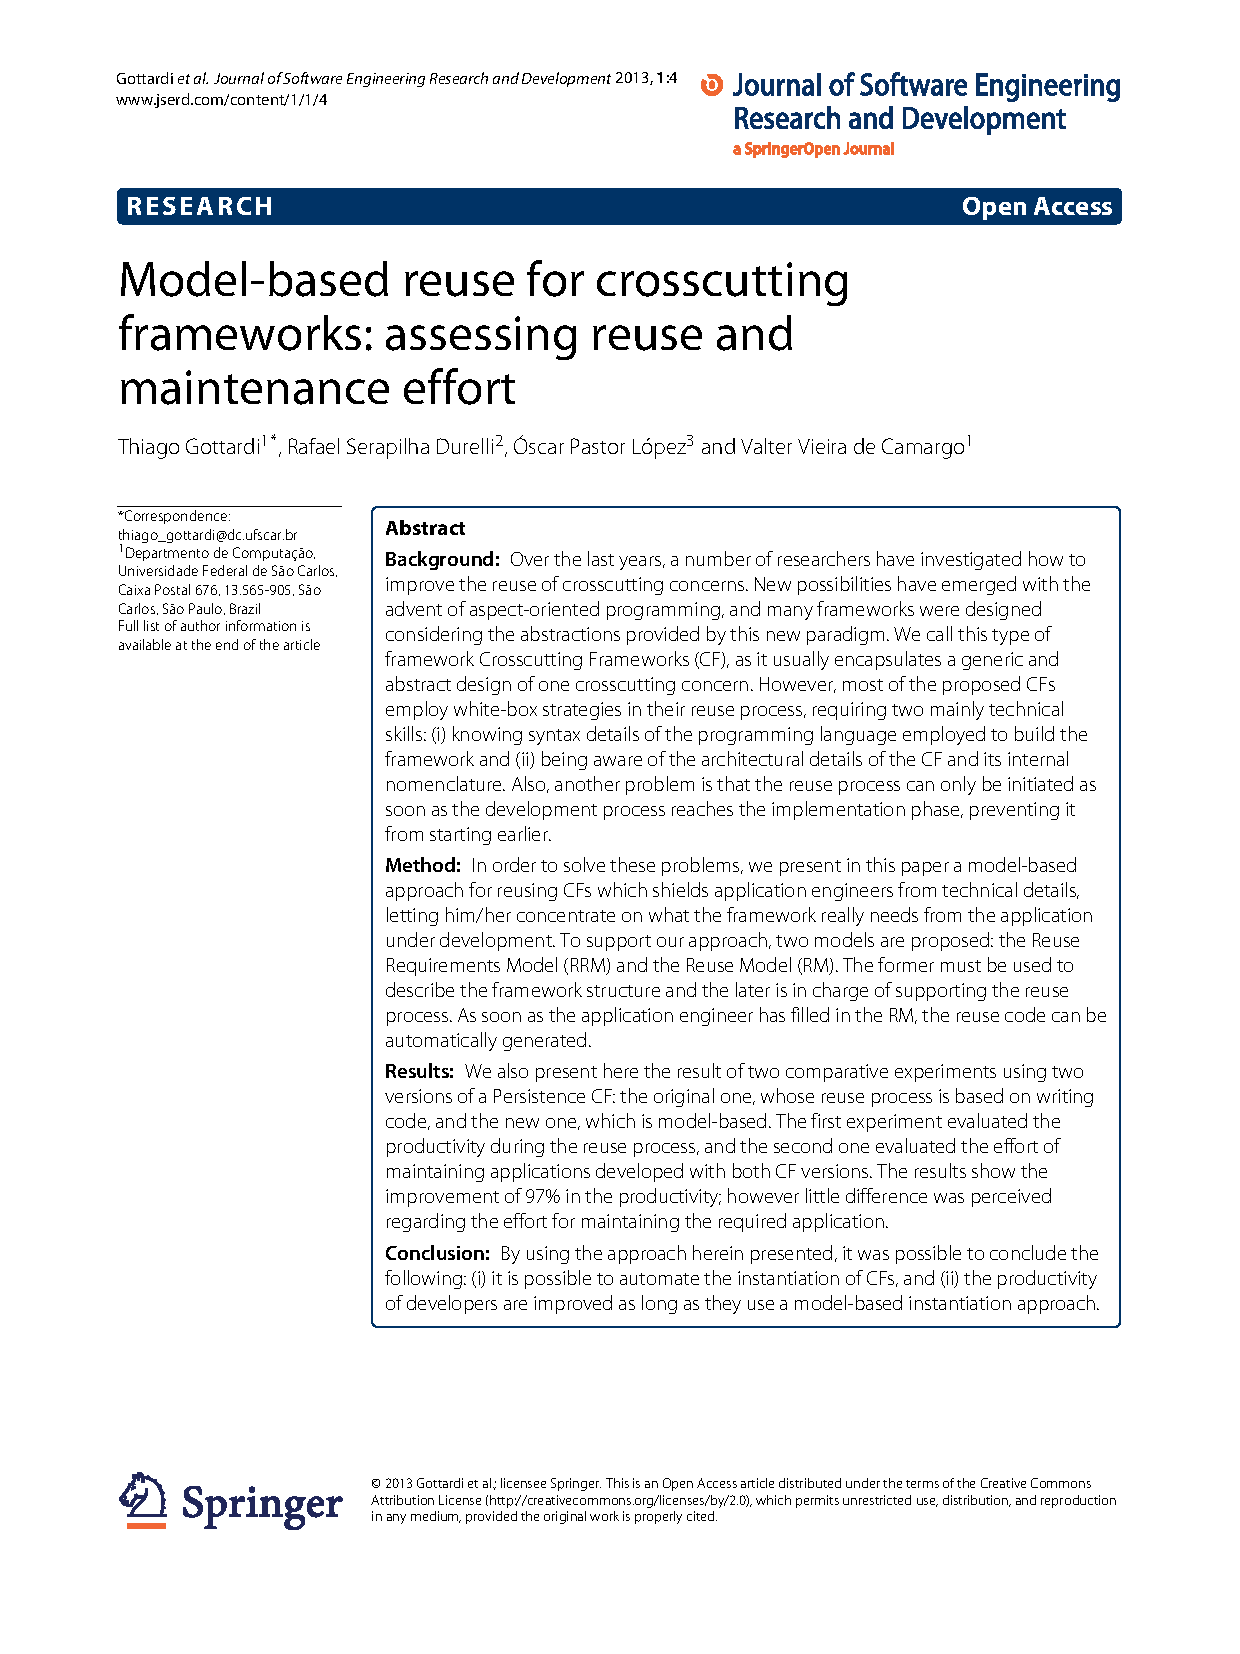
\includepdf[pages={-}]{apendices/ArtigosRelatorio/Model_based_reuse_for_crosscutting_frameworks_assessing_reuse_and_maintenance_effort.pdf}

%--------anexo 2---------------------------------------------------------------

\subsection*{Anexo 2: Comprovante da publicação no \emph{International Conference on Information Reuse and Integration} (IRI'13)} \label{anexo:comprovante_IRI_TEUS}

\begin{itemize}
	\item Uma cópia do artigo é apresentado a seguir (a partir da próxima página).
\end{itemize}
\clearpage
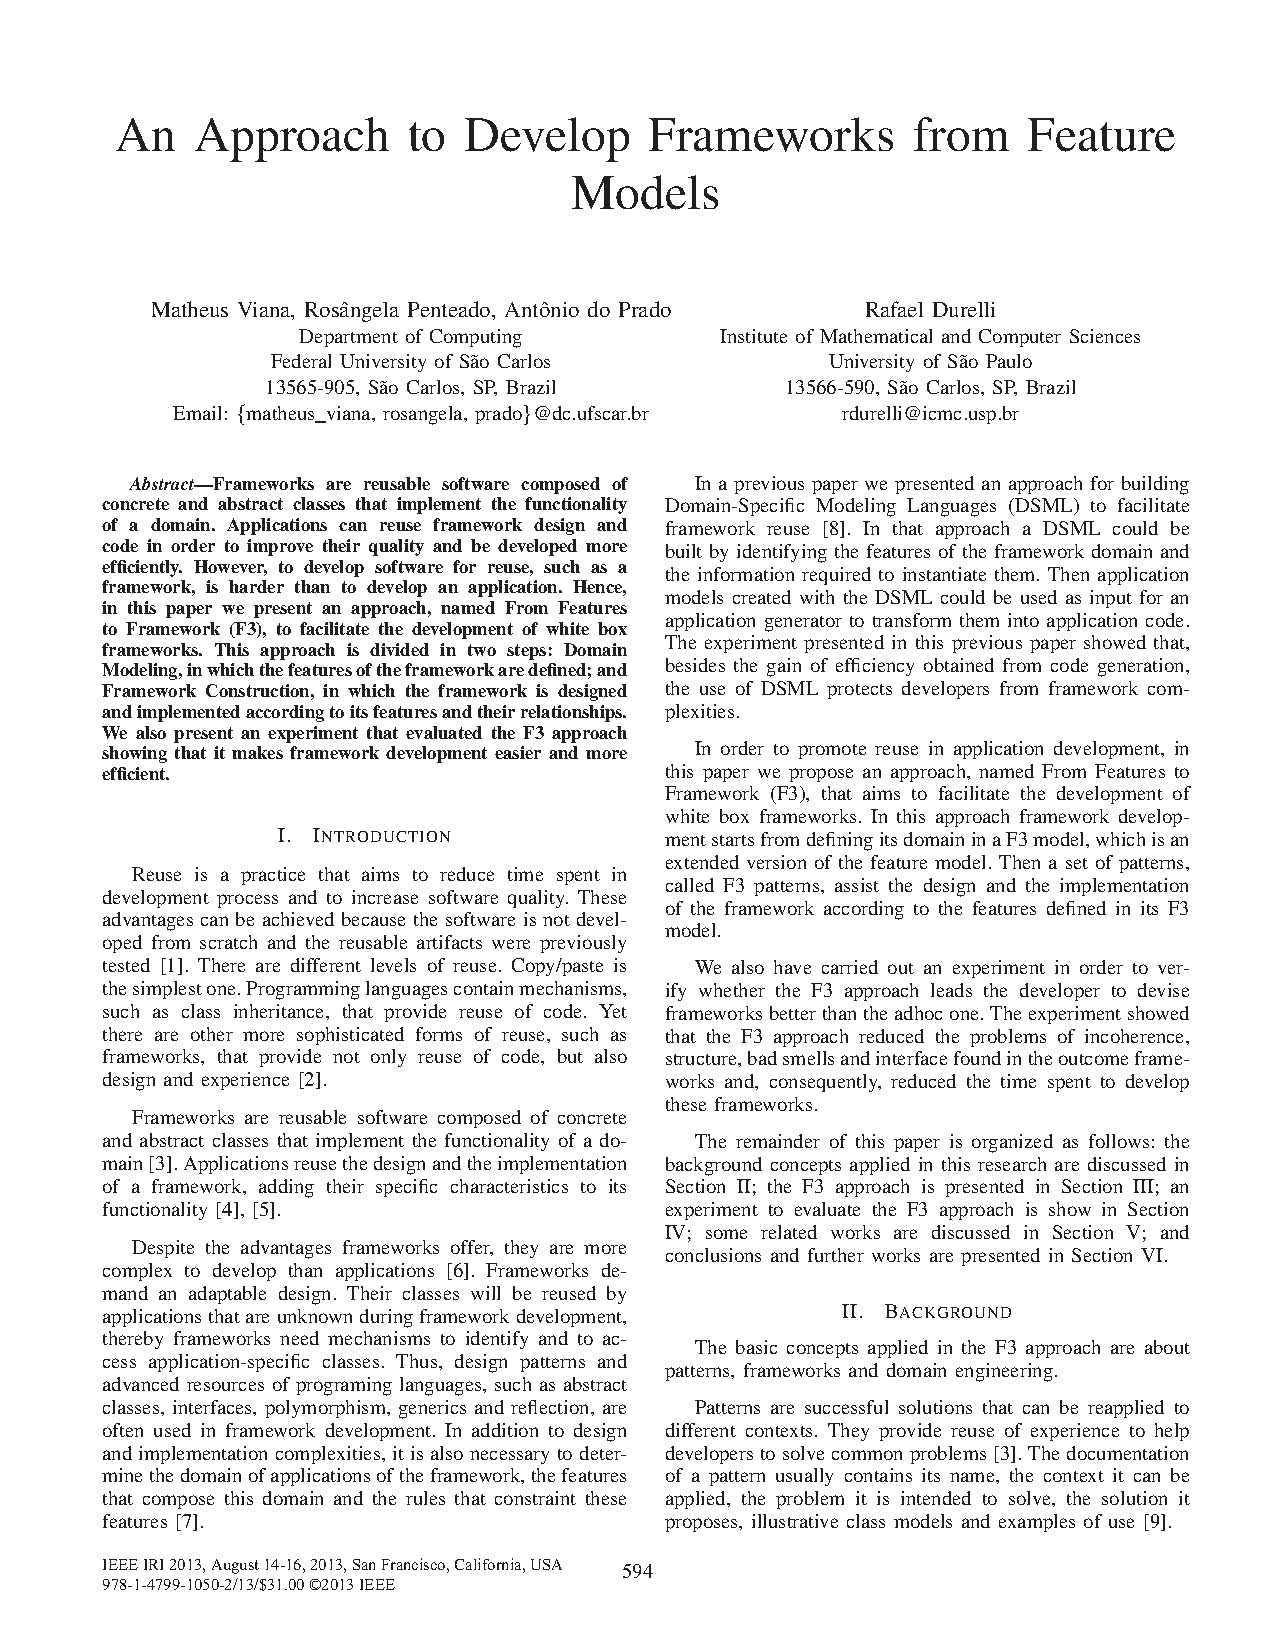
\includepdf[pages={-}]{apendices/ArtigosRelatorio/An_Approach_to_Develop_Frameworks_from_Feature_Models.pdf}

%--------anexo 3---------------------------------------------------------------

\subsection*{Anexo 3: Comprovante da publicação no \emph{Simpósio Brasileiro de Engenharia de Software} (SBES'13)} \label{anexo:comprovante_SBES_13}

\begin{itemize}
	\item Uma cópia do artigo é apresentado a seguir (a partir da próxima página).
\end{itemize}
\clearpage
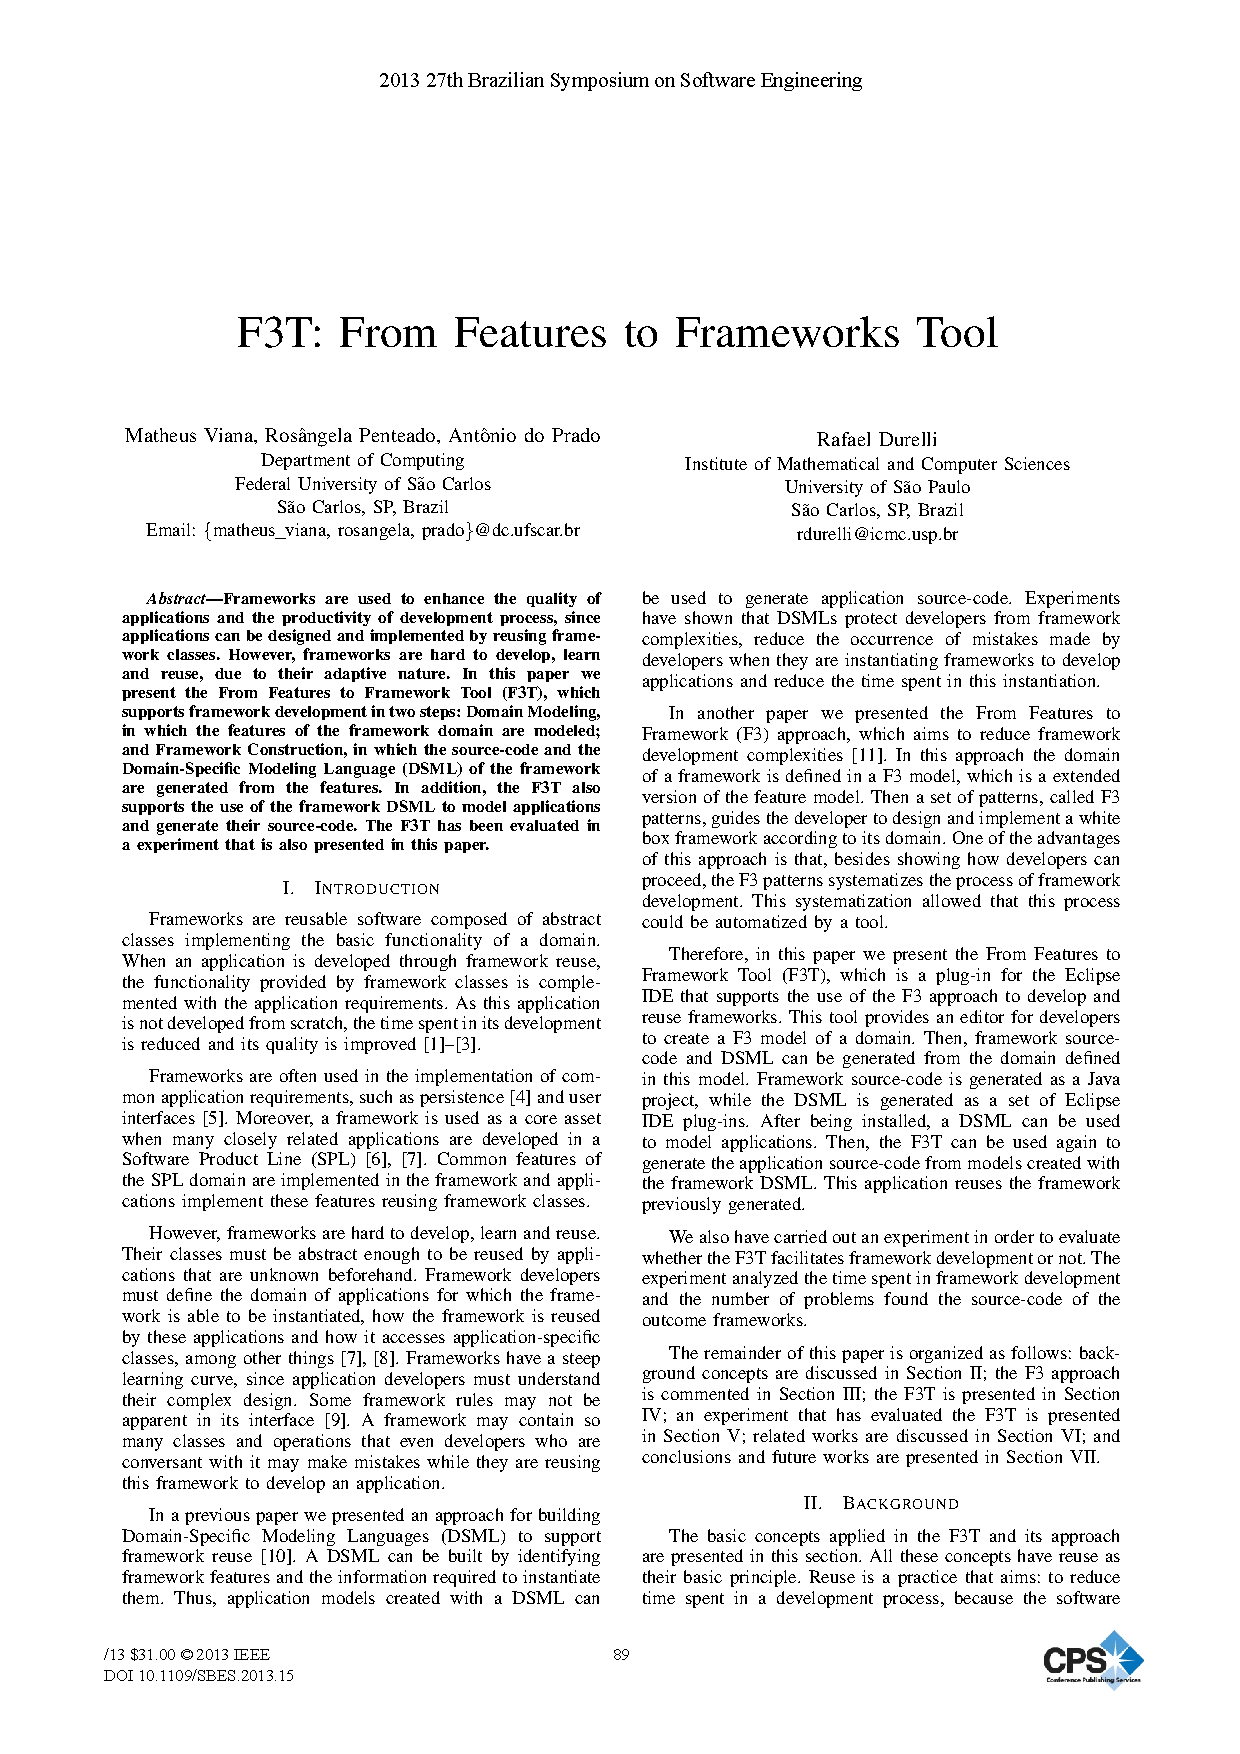
\includepdf[pages={-}]{apendices/ArtigosRelatorio/F3T_From_Features_to_Frameworks_Tool.pdf}

%--------anexo 4---------------------------------------------------------------

\subsection*{Anexo 4: Comprovante da publicação no \emph{Latin American Workshop on Aspect-Oriented Software Development} (LA-WASP)} \label{anexo:comprovante_LA_WASP}

\begin{itemize}
	\item Uma cópia do artigo é apresentado a seguir (a partir da próxima página).
\end{itemize}
\clearpage
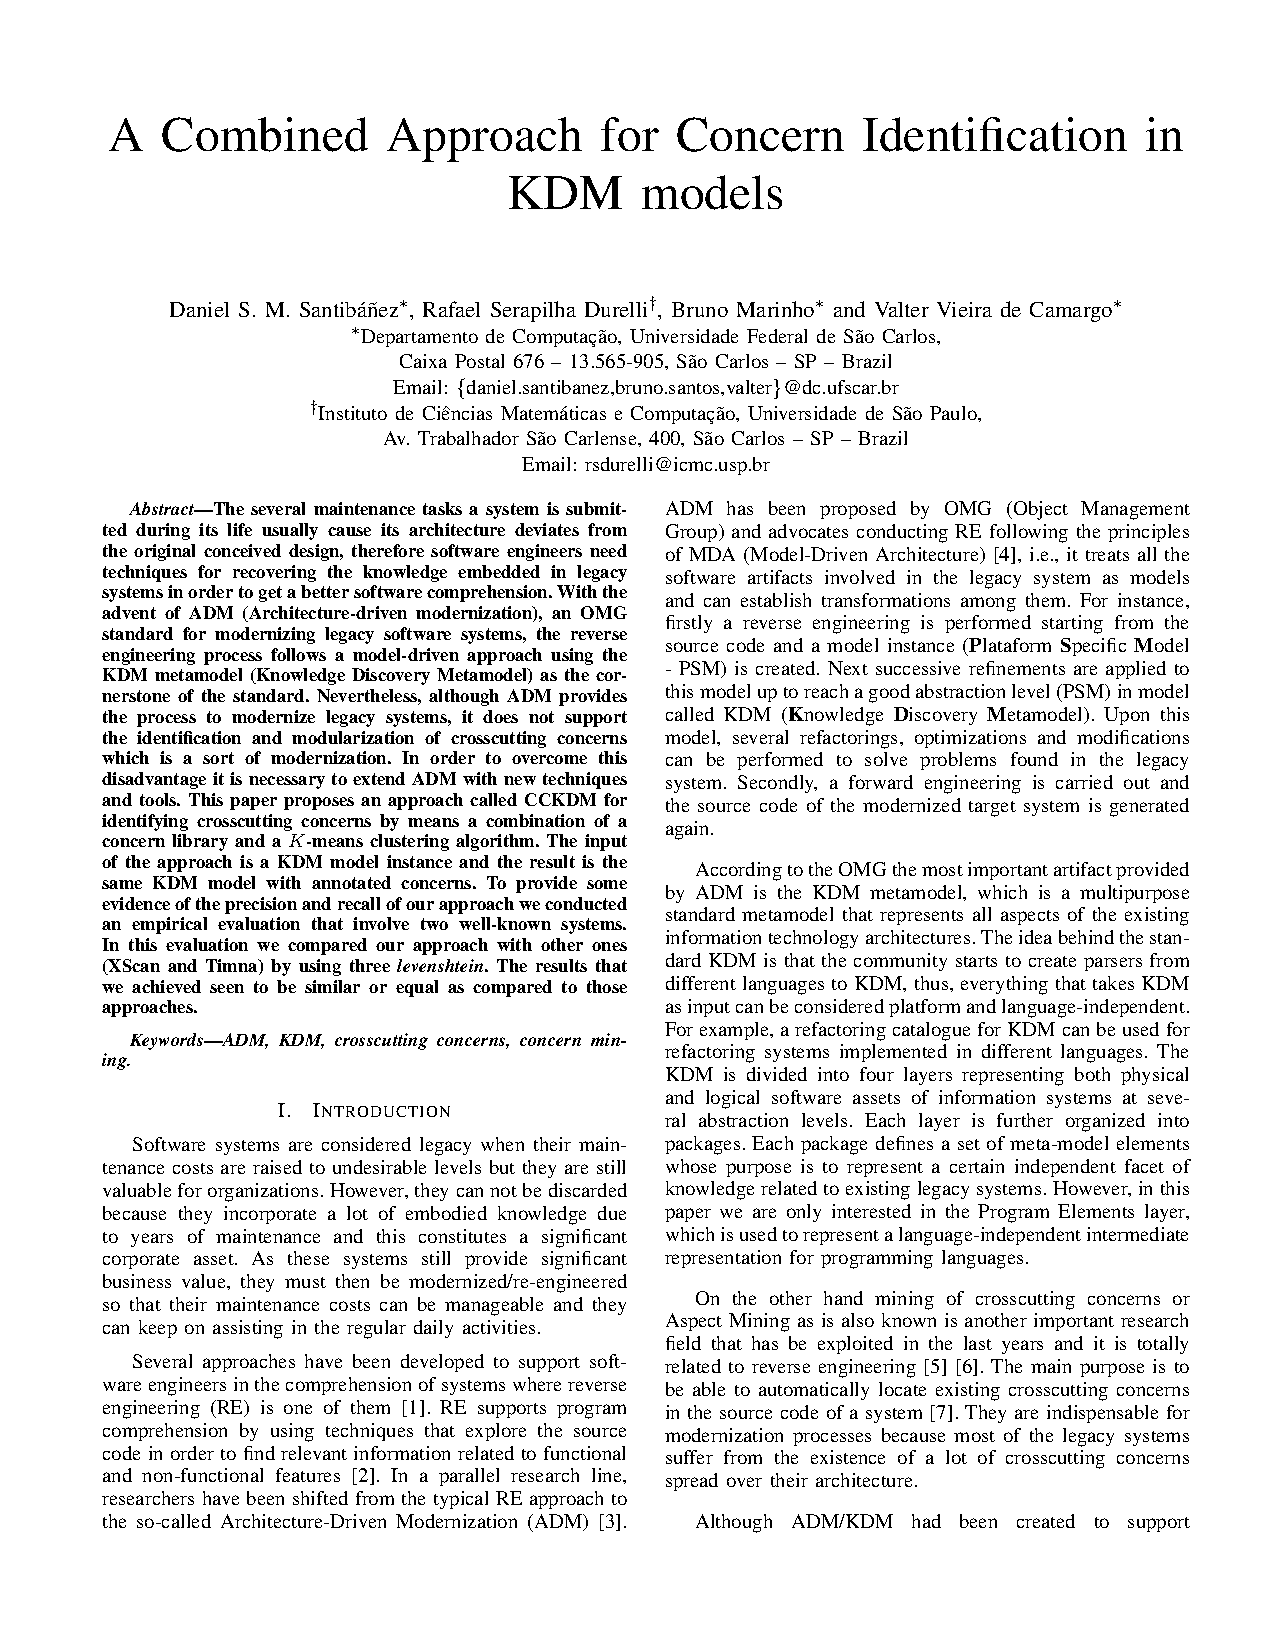
\includepdf[pages={-}]{apendices/ArtigosRelatorio/A_Combined_Approach_for_Concern_Identification_in_KDM_models.pdf}

%--------anexo 5---------------------------------------------------------------

\subsection*{Anexo 5: Comprovante da publicação no \emph{The 14th International Conference on Computational Science and Applications} (ICCSA 2014)} \label{anexo:comprovante_ICCSA}

\begin{itemize}
	\item Uma cópia do artigo é apresentado a seguir (a partir da próxima página).
\end{itemize}
\clearpage
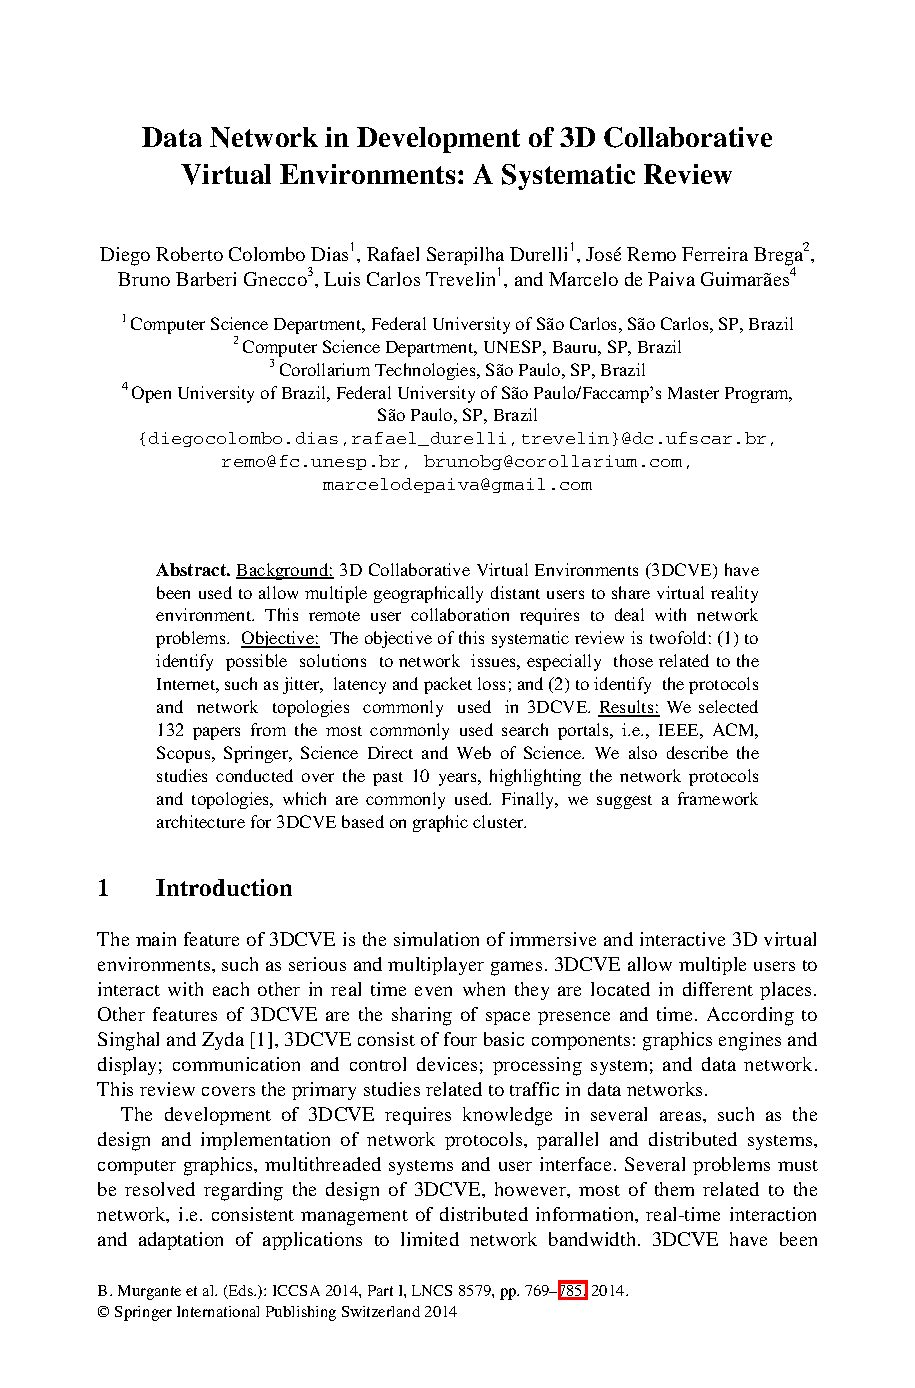
\includepdf[pages={-}]{apendices/ArtigosRelatorio/Data_Network_in_Development_of_D_Collaborative_Virtual_Environments_A_Systematic_Review.pdf}

%--------anexo 6---------------------------------------------------------------

\subsection*{Anexo 6: Comprovante da publicação no \emph{IEEE International Conference on Information Reuse and Integration 2014} (IRI 2014)} \label{anexo:comprovante_IRI_Rafael}

\begin{itemize}
	\item Uma cópia do artigo é apresentado a seguir (a partir da próxima página).
\end{itemize}
\clearpage
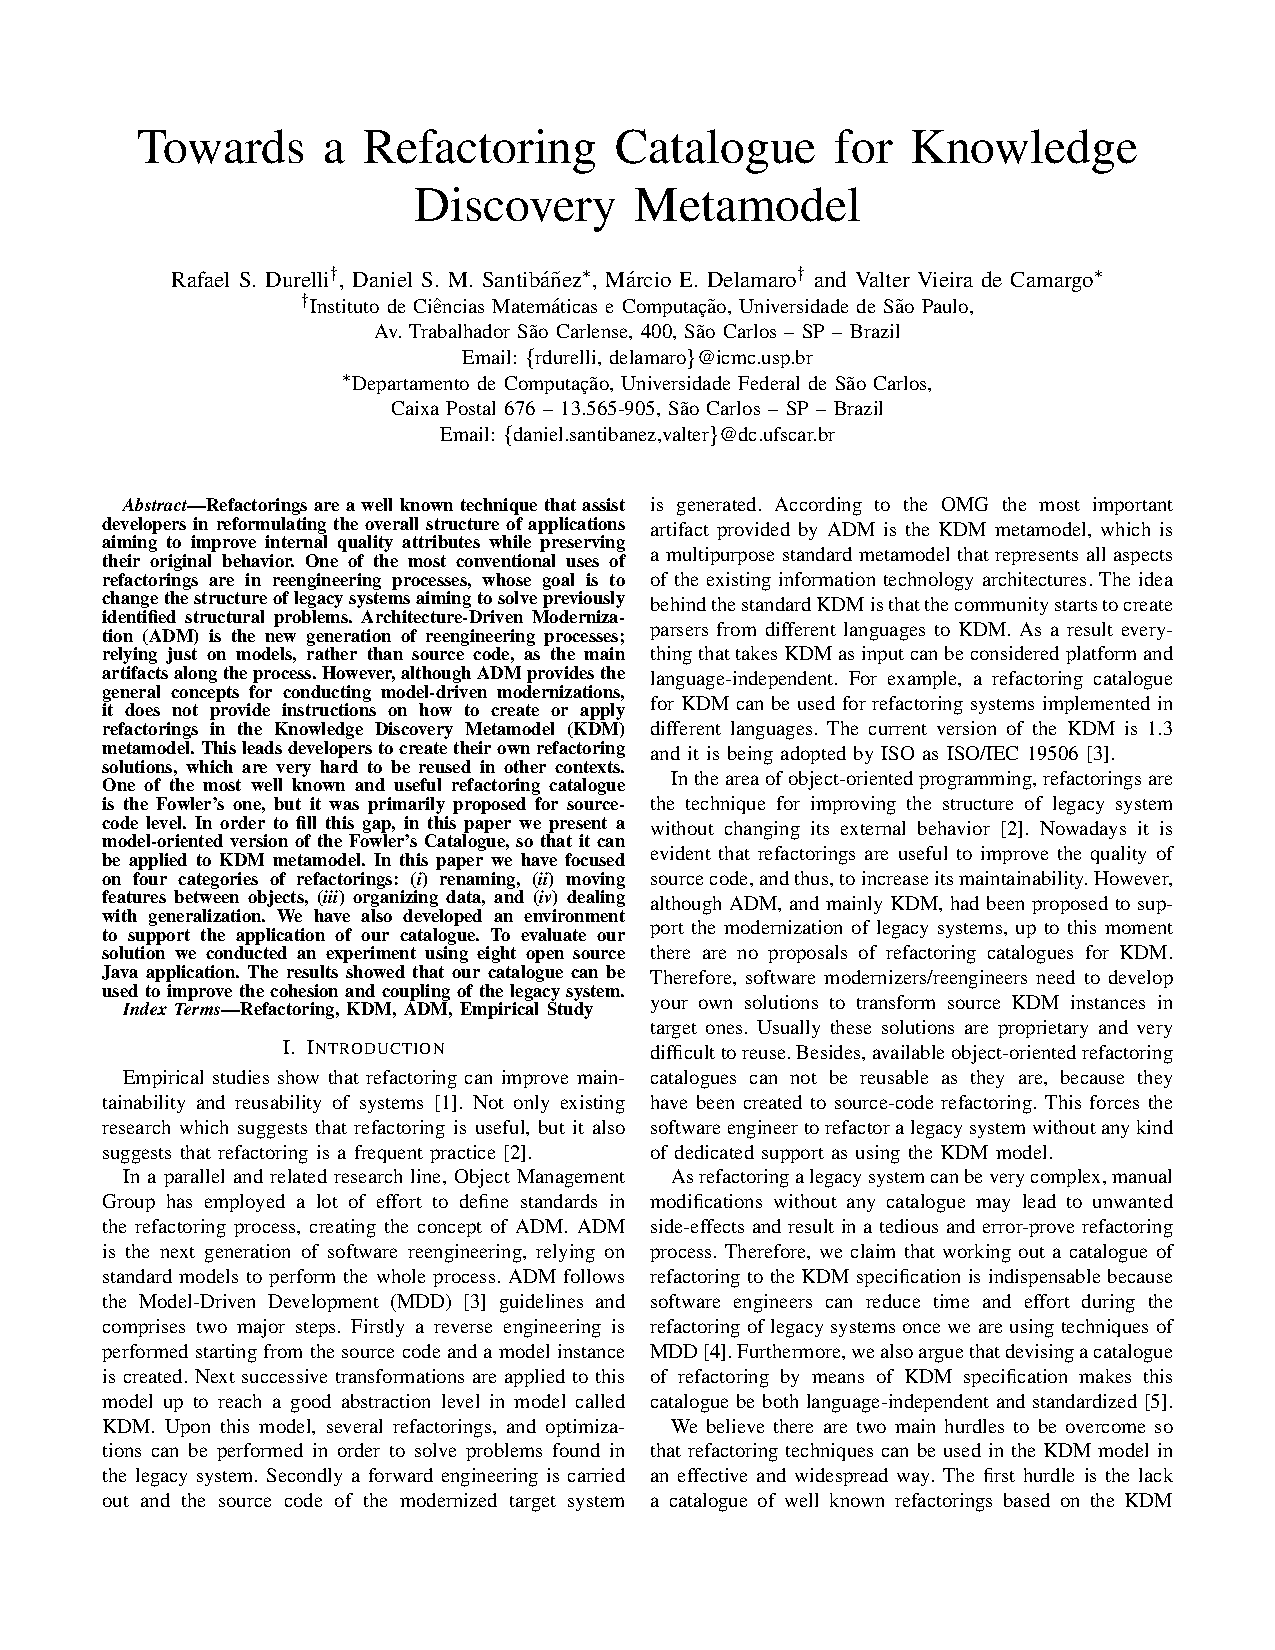
\includepdf[pages={-}]{apendices/ArtigosRelatorio/ieee_IRI_2014_camera_ready.pdf}

%--------anexo 7---------------------------------------------------------------

\subsection*{Anexo 7: Comprovante da publicação no \emph{IEEE International Conference on Information Reuse and Integration 2014} (IRI 2014)} \label{anexo:comprovante_IRI_Rafael_map}

\begin{itemize}
	\item Uma cópia do artigo é apresentado a seguir (a partir da próxima página).
\end{itemize}
\clearpage
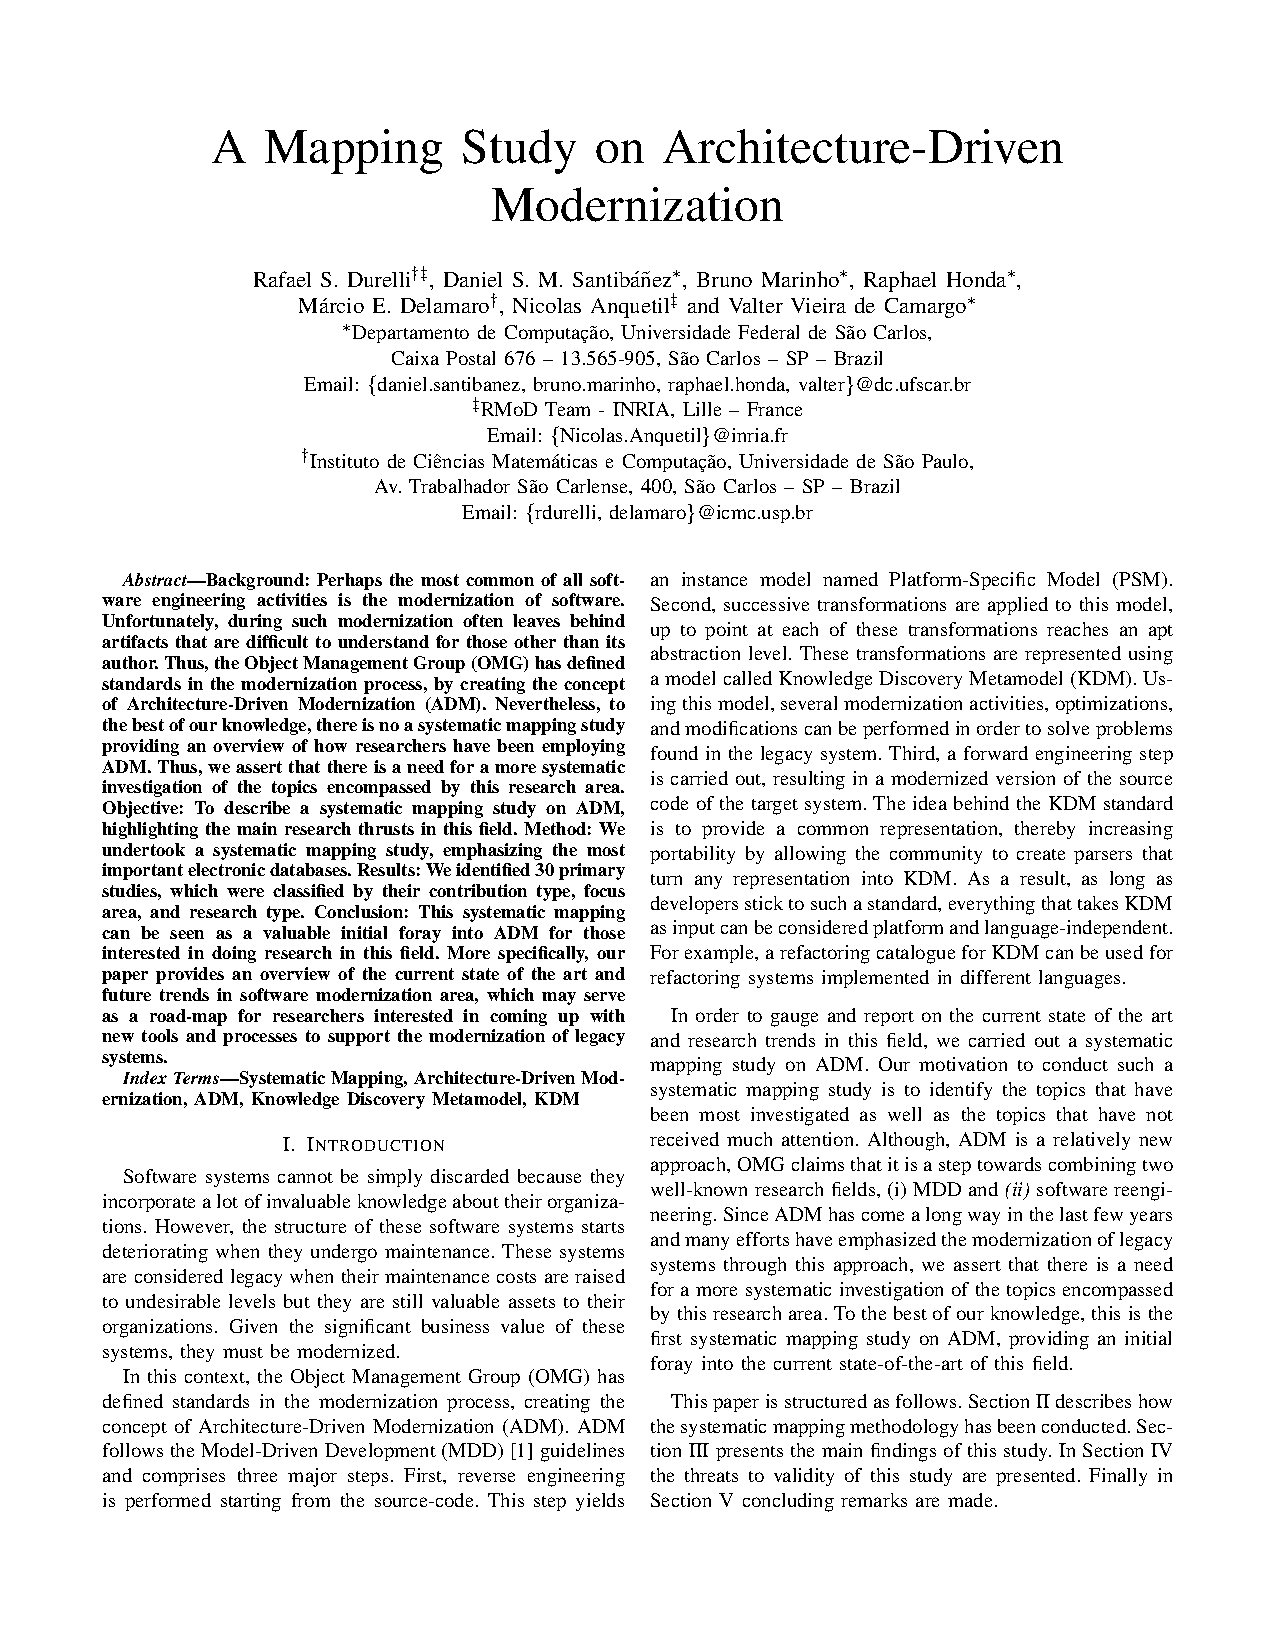
\includepdf[pages={-}]{apendices/ArtigosRelatorio/ieee_iri_mapeamento_systematic_camera_ready.pdf}

%--------anexo 8---------------------------------------------------------------

\subsection*{Anexo 8: Comprovante da publicação no \emph{28th Brazilian Symposium on Software Engineering } (SBES 2014)} \label{anexo:comprovante_SBES_Marinho}

\begin{itemize}
	\item Uma cópia do artigo é apresentado a seguir (a partir da próxima página).
\end{itemize}
\clearpage
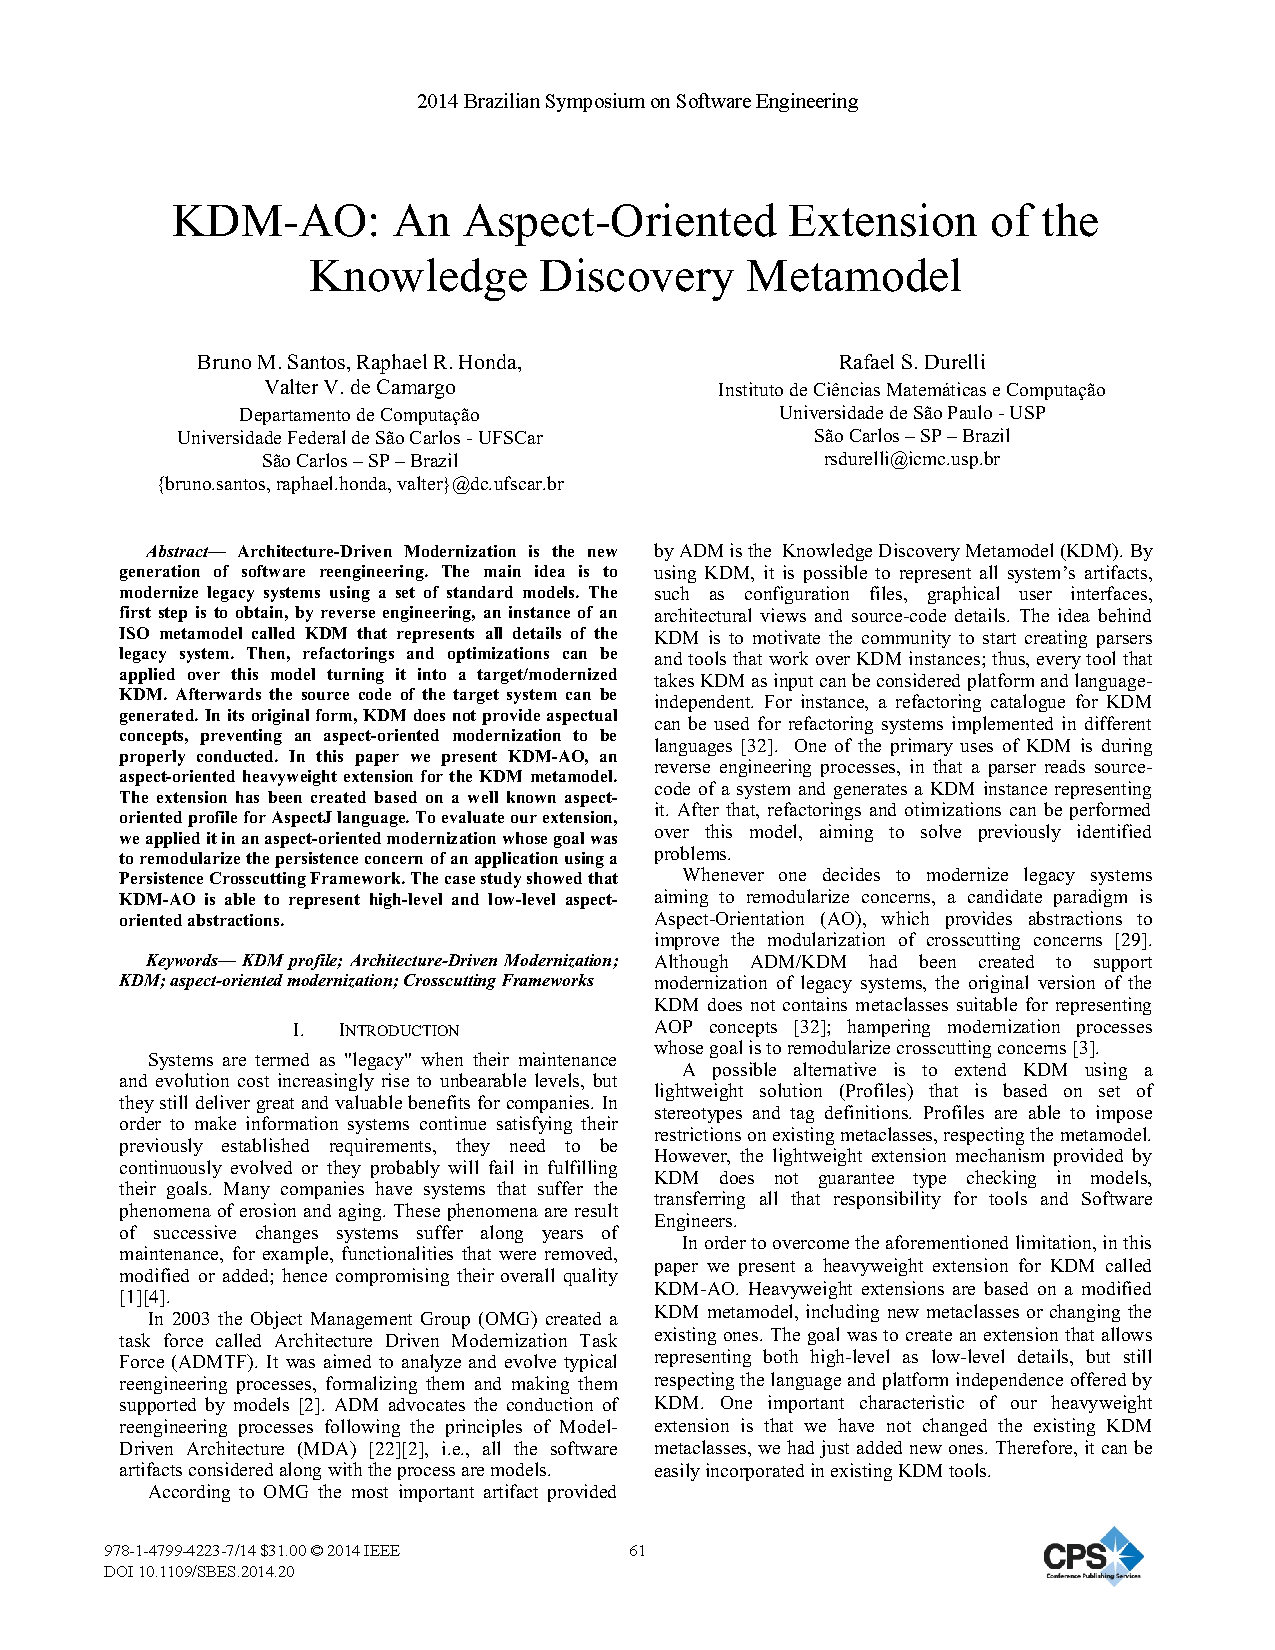
\includepdf[pages={-}]{apendices/ArtigosRelatorio/KDM_AO_An_Aspect_Oriented_Extension_of_the_Knowledge_Discovery_Metamodel.pdf}

%--------anexo 9---------------------------------------------------------------

\subsection*{Anexo 9: Comprovante da publicação no \emph{II Workshop on Software Visualization, Evolution and Maintenance -- Brazilian Conference on Software: theory and practice, 2014 } (VEM 2014)} \label{anexo:comprovante_VEM}

\begin{itemize}
	\item Uma cópia do artigo é apresentado a seguir (a partir da próxima página).
\end{itemize}
\clearpage
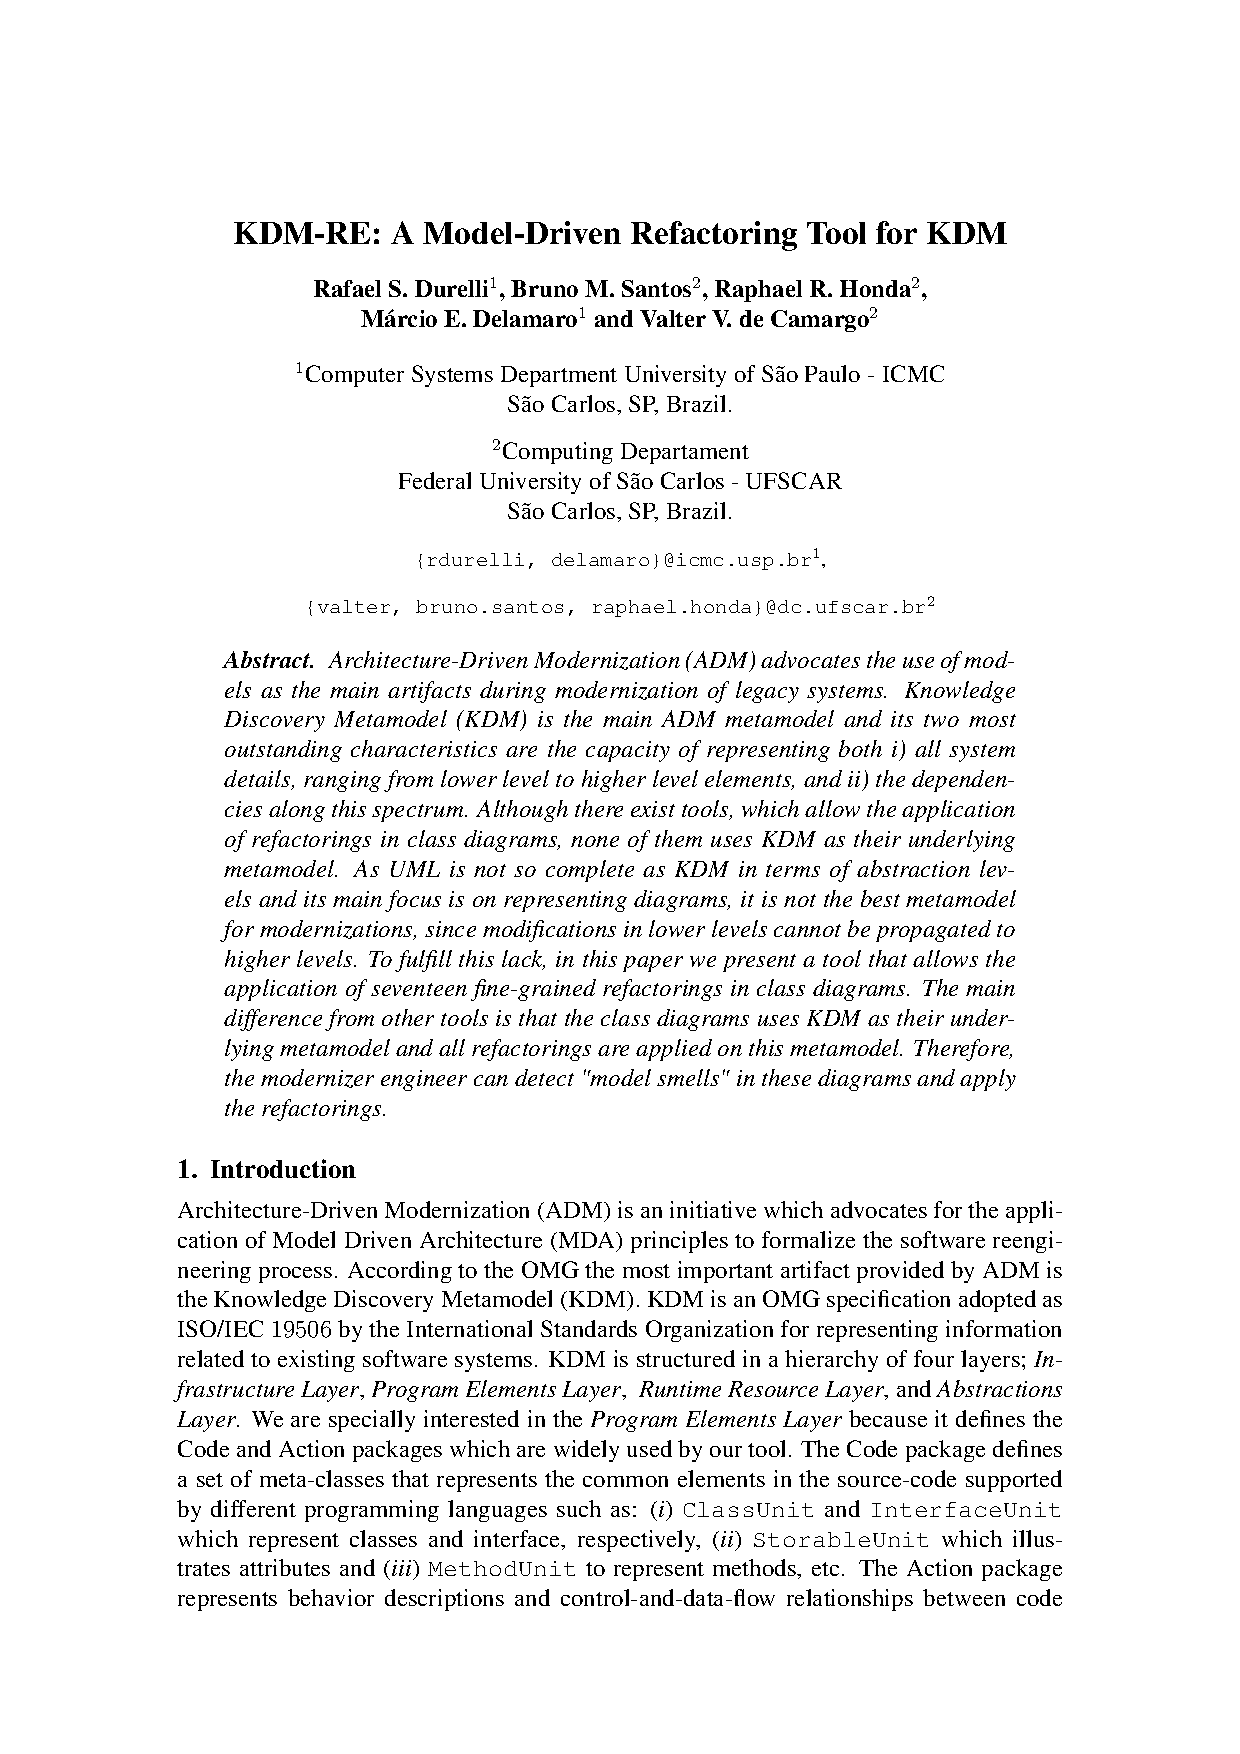
\includepdf[pages={-}]{apendices/ArtigosRelatorio/KDM-RE.pdf}

%--------anexo 10---------------------------------------------------------------

\subsection*{Anexo 10: Comprovante da publicação no \emph{International Conference on Enterprise Information Systems, 2013 } (ICEIS 2013)} \label{anexo:comprovante_ICEIS_paulo}

\begin{itemize}
	\item Uma cópia do artigo é apresentado a seguir (a partir da próxima página).
\end{itemize}
\clearpage
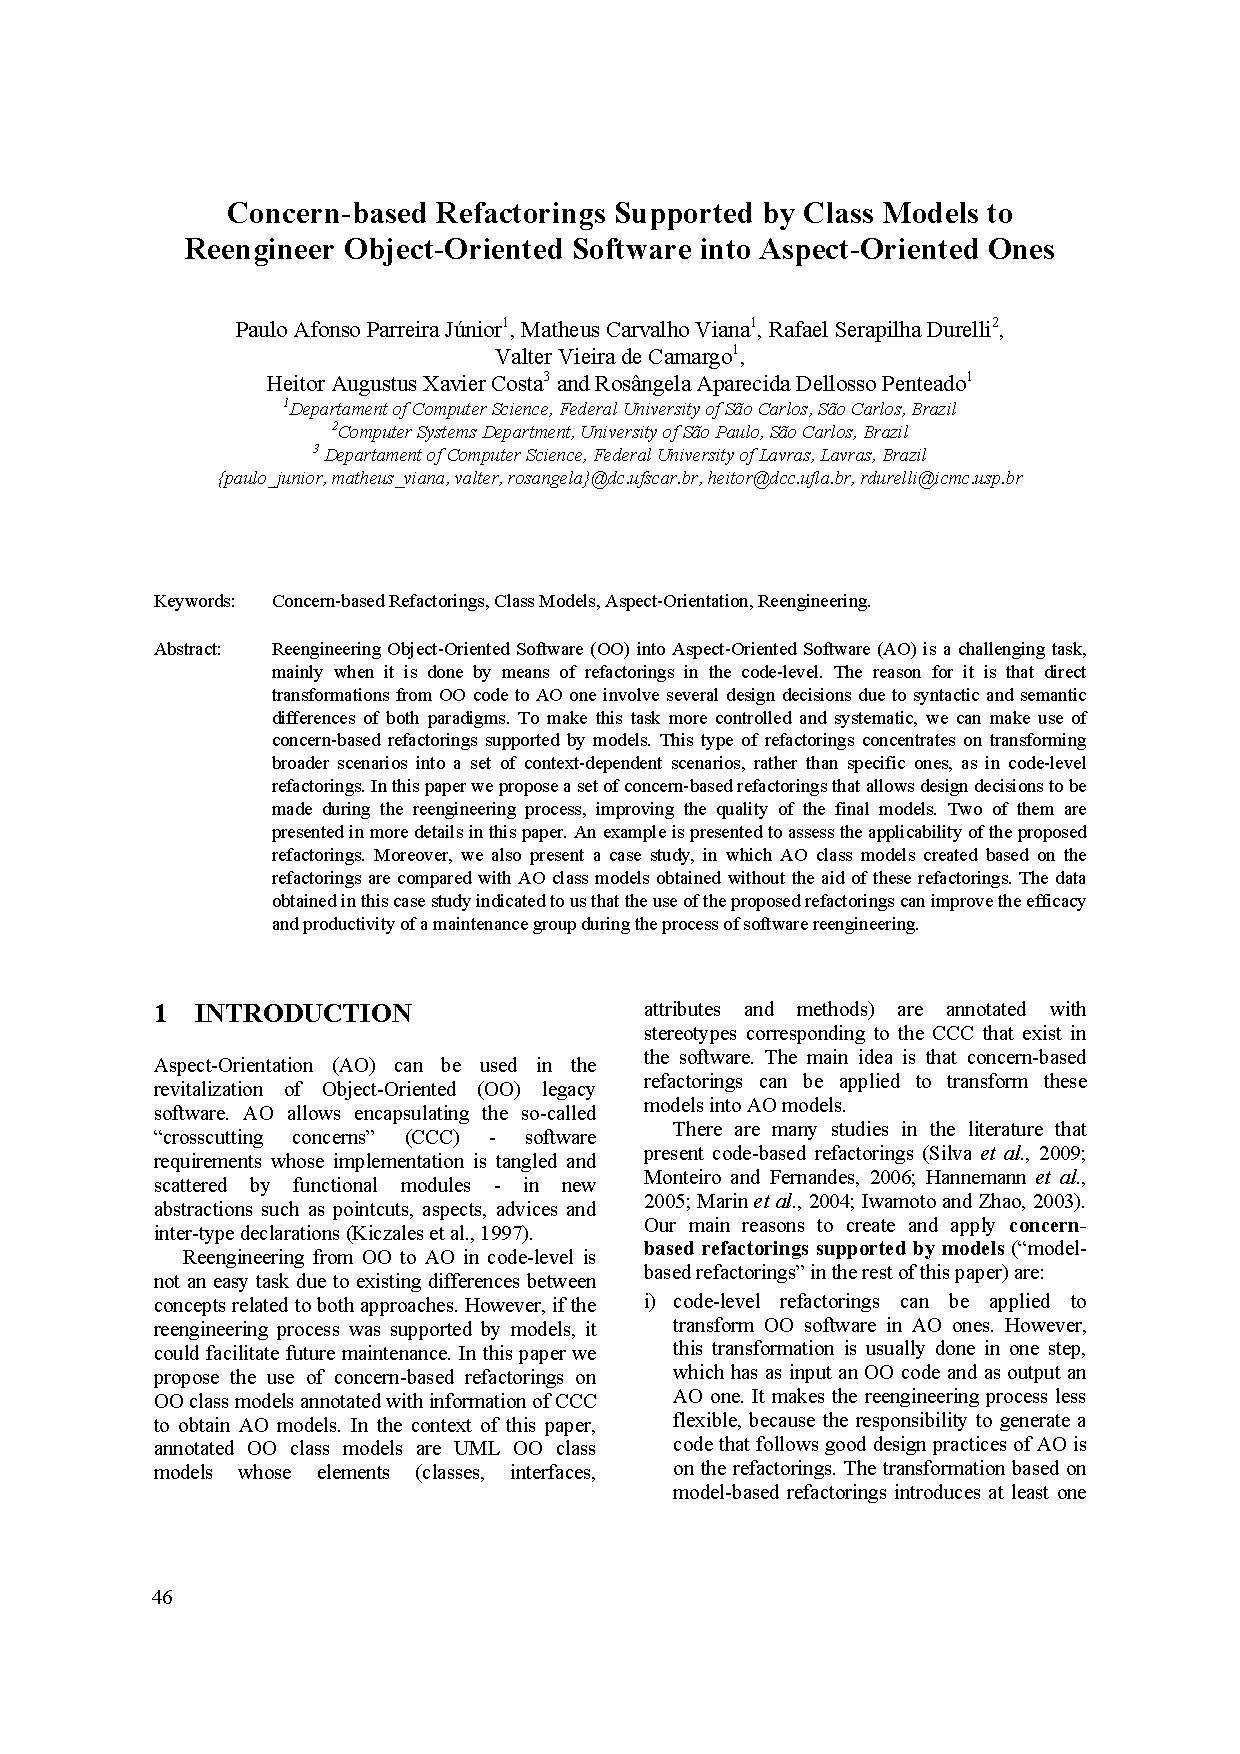
\includepdf[pages={-}]{apendices/ArtigosRelatorio/Concern_based_Refactorings_Supported_by_Class_Models_to_Reengineer_Object_Oriented_Software_into_Aspect-Oriented_Ones.pdf}

%--------anexo 11---------------------------------------------------------------

\subsection*{Anexo 11: Comprovante da publicação no \emph{11th Workshop on Software Modularity (WMod) -- Brazilian Conference on Software: theory and practice } (WMod 2014)} \label{anexo:comprovante_WMOD}

\begin{itemize}
	\item Uma cópia do artigo é apresentado a seguir (a partir da próxima página).
\end{itemize}
\clearpage
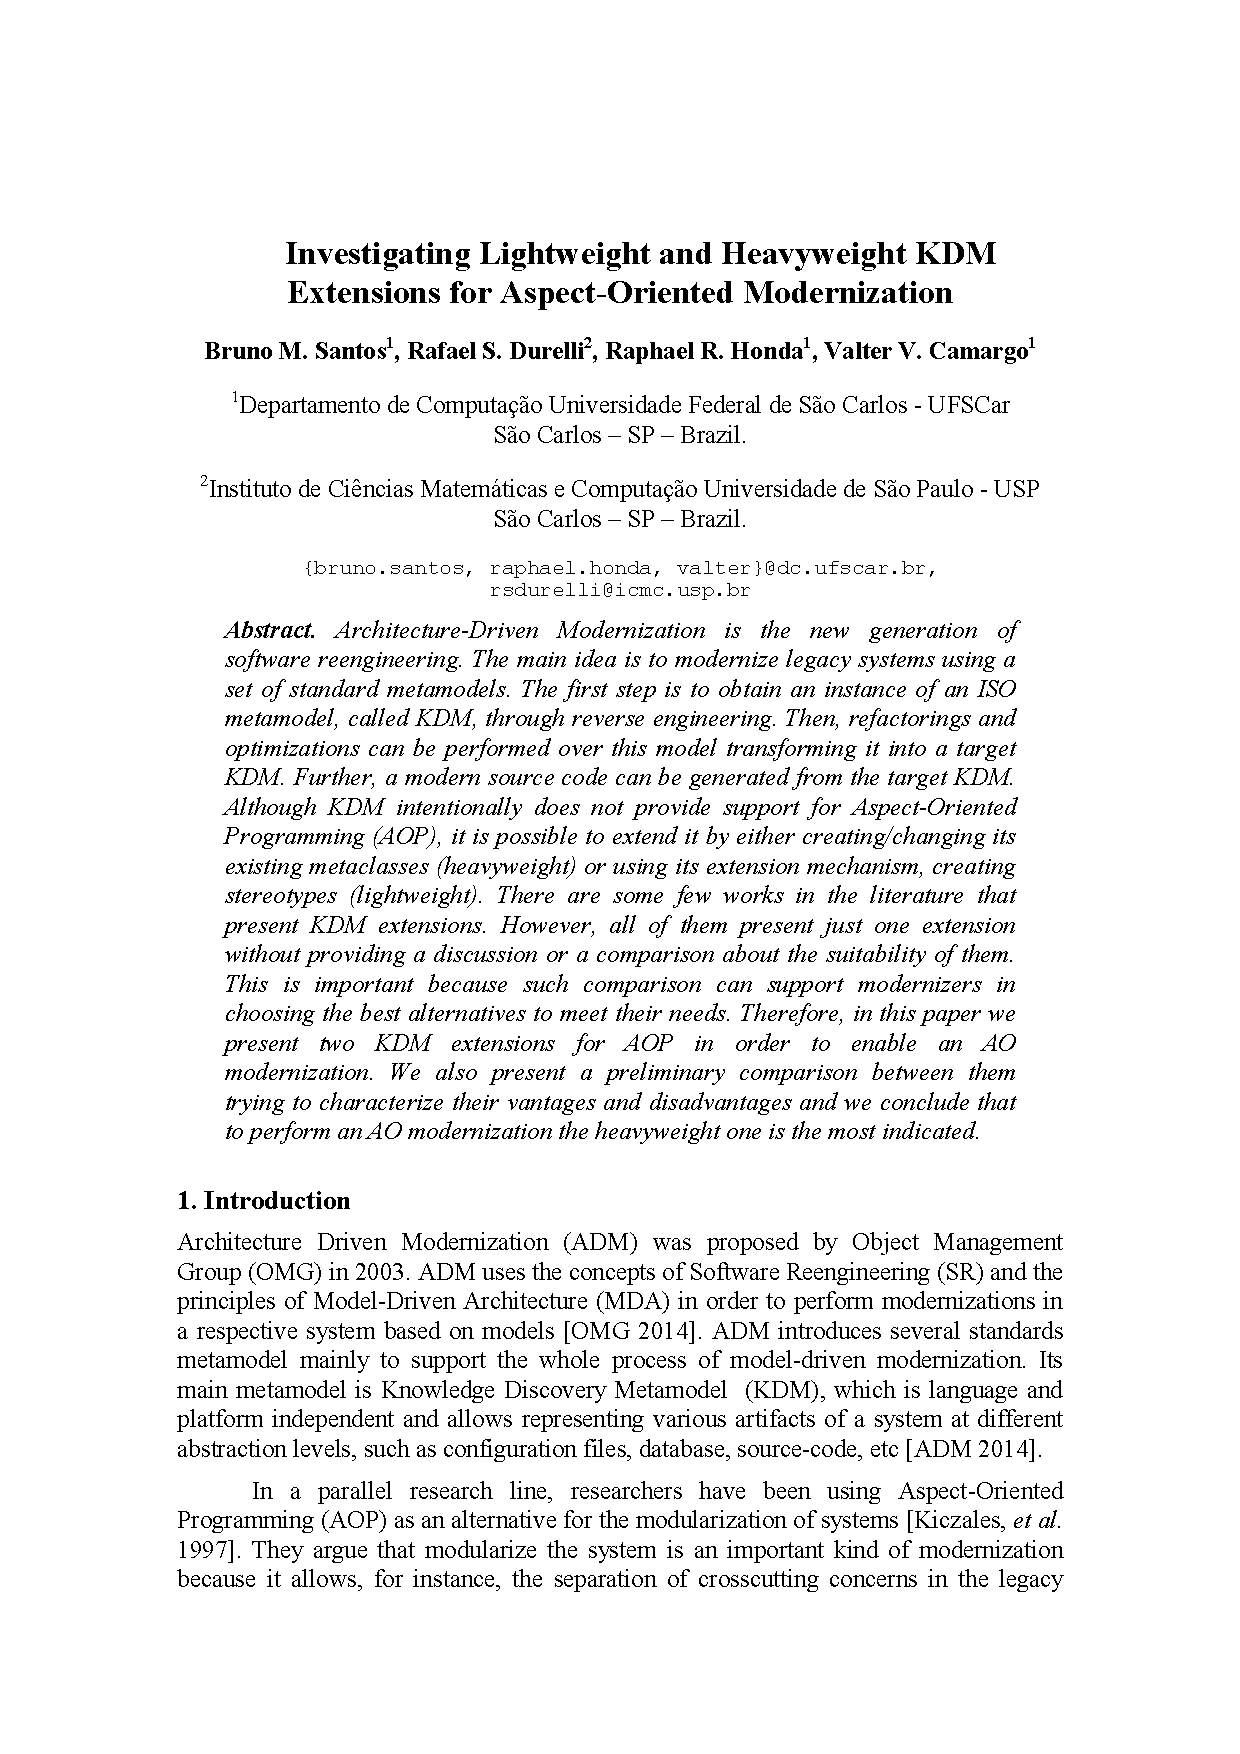
\includepdf[pages={-}]{apendices/ArtigosRelatorio/WMod_BRUNO.pdf}

%--------anexo 12---------------------------------------------------------------
\subsection*{Anexo 12: Carta do orientador estrangeiro atestando a realização das atividades} \label{anexo:comprovante_nicolas}
\begin{itemize}
	\item A carta é apresentado a seguir (a partir da próxima página).
\end{itemize}
\clearpage
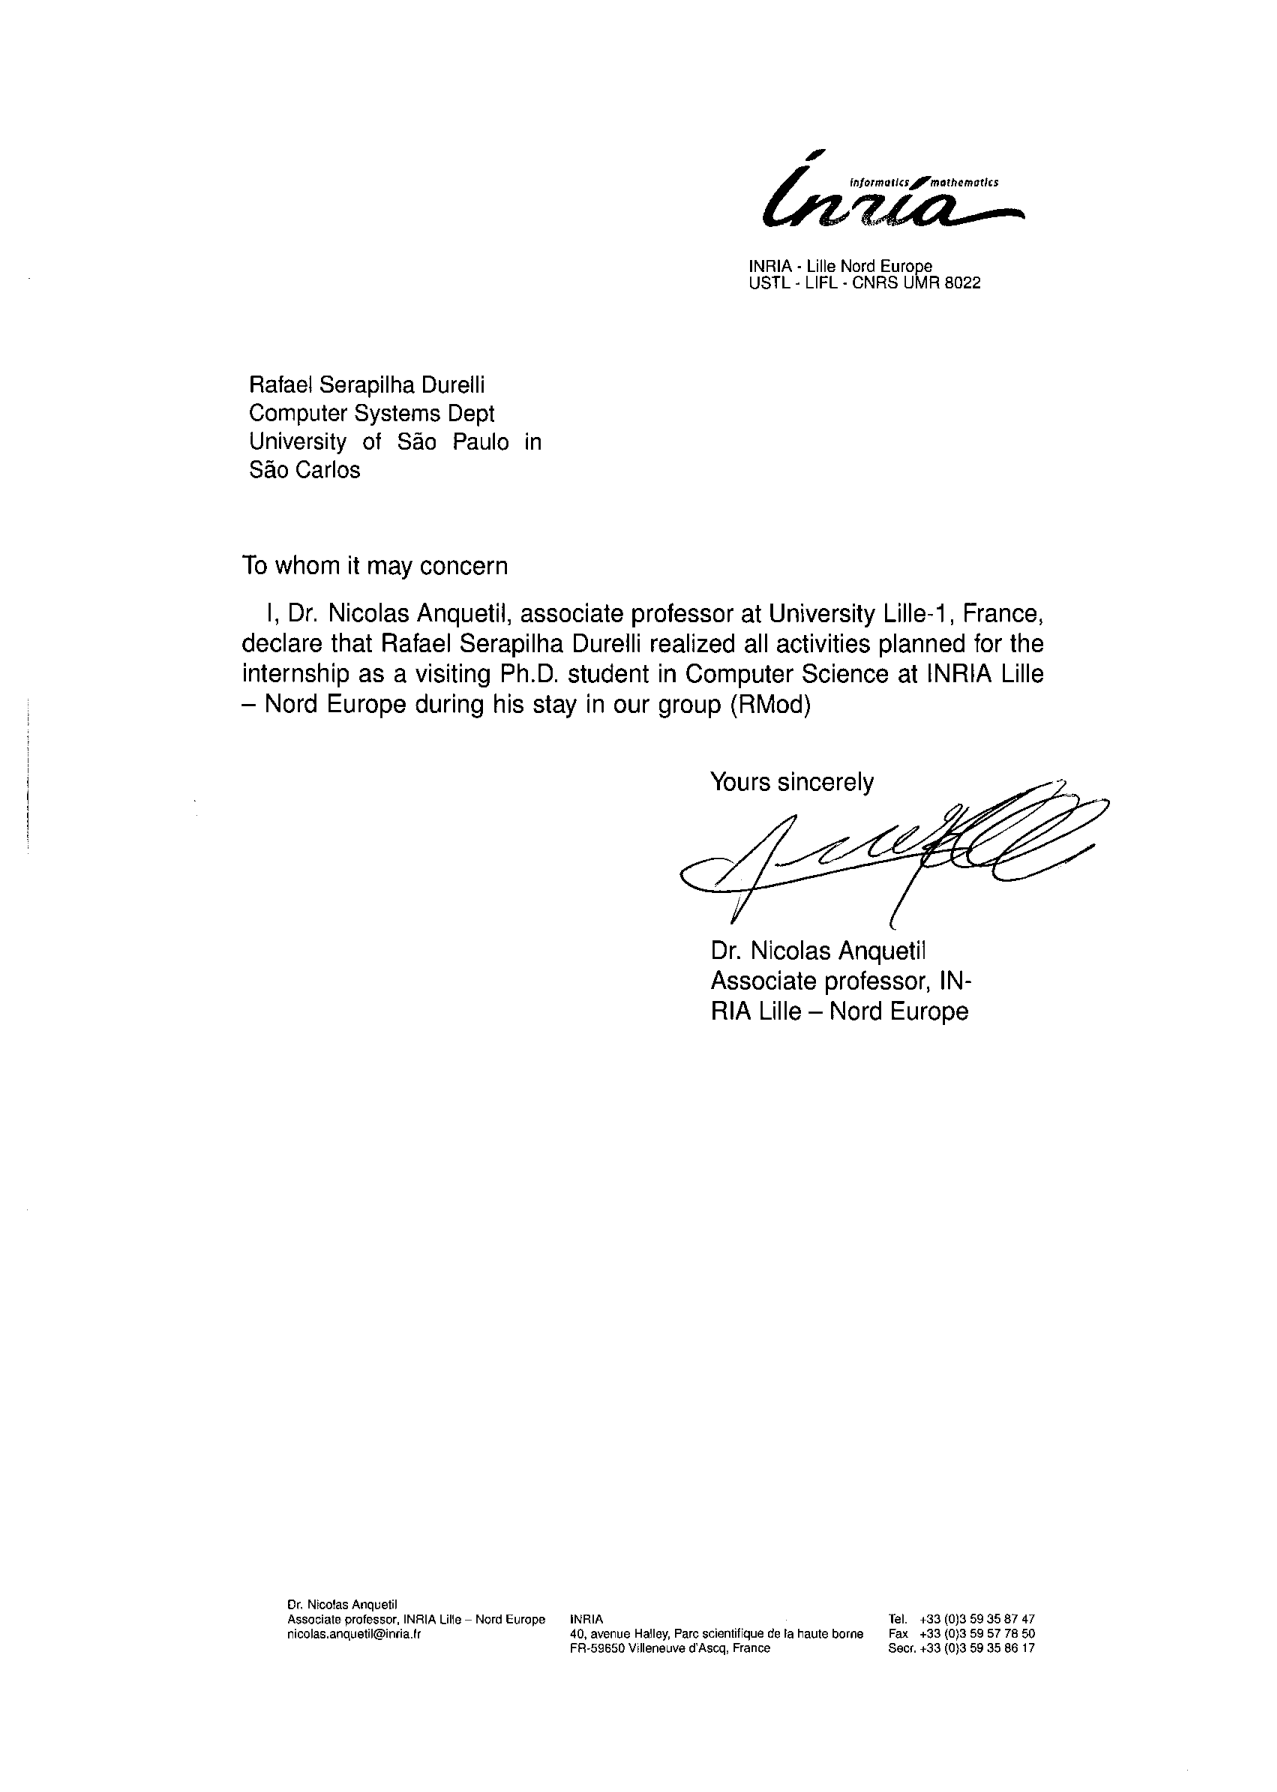
\includepdf[pages={-}]{apendices/NicolasAssinatura.pdf}

\end{document}
